\documentclass[a4paper,
fontsize=11pt,
%headings=small,
oneside,
numbers=noperiodatend,
parskip=half-,
bibliography=totoc,
final
]{scrartcl}

\usepackage[babel]{csquotes}
\usepackage{synttree}
\usepackage{graphicx}
\setkeys{Gin}{width=.4\textwidth} %default pics size

\graphicspath{{./plots/}}
\usepackage[ngerman]{babel}
\usepackage[T1]{fontenc}
%\usepackage{amsmath}
\usepackage[utf8x]{inputenc}
\usepackage[hyphens]{url}
\usepackage{xurl}
\usepackage{booktabs} 
\usepackage[left=2.4cm,right=2.4cm,top=2.3cm,bottom=2cm,includeheadfoot]{geometry}
\usepackage{eurosym}
\usepackage{multirow}
\usepackage[ngerman]{varioref}
\setcapindent{1em}
\renewcommand{\labelitemi}{--}
\usepackage{paralist}
\usepackage{pdfpages}
\usepackage{lscape}
\usepackage{float}
\usepackage{acronym}
\usepackage{eurosym}
\usepackage{longtable,lscape}
\usepackage{mathpazo}
\usepackage[normalem]{ulem} %emphasize weiterhin kursiv
\usepackage[flushmargin,ragged]{footmisc} % left align footnote
\usepackage{ccicons} 
\setcapindent{0pt} % no indentation in captions

%%%% fancy LIBREAS URL color 
\usepackage{xcolor}
\definecolor{libreas}{RGB}{112,0,0}

\usepackage{listings}

\urlstyle{same}  % don't use monospace font for urls

\usepackage[fleqn]{amsmath}

%adjust fontsize for part

\usepackage{sectsty}
\partfont{\large}

%Das BibTeX-Zeichen mit \BibTeX setzen:
\def\symbol#1{\char #1\relax}
\def\bsl{{\tt\symbol{'134}}}
\def\BibTeX{{\rm B\kern-.05em{\sc i\kern-.025em b}\kern-.08em
    T\kern-.1667em\lower.7ex\hbox{E}\kern-.125emX}}

\usepackage{fancyhdr}
\fancyhf{}
\pagestyle{fancyplain}
\fancyhead[R]{\thepage}

% make sure bookmarks are created eventough sections are not numbered!
% uncommend if sections are numbered (bookmarks created by default)
\makeatletter
\renewcommand\@seccntformat[1]{}
\makeatother

% typo setup
\clubpenalty = 10000
\widowpenalty = 10000
\displaywidowpenalty = 10000

\usepackage{hyperxmp}
\usepackage[colorlinks, linkcolor=black,citecolor=black, urlcolor=libreas,
breaklinks= true,bookmarks=true,bookmarksopen=true]{hyperref}
\usepackage{breakurl}

%meta
%meta

\fancyhead[L]{U. Wimmer\\ %author
LIBREAS. Library Ideas, 37 (2020). % journal, issue, volume.
\href{https://doi.org/10.18452/21540}{\color{black}https://doi.org/10.18452/21540}
{}} % doi 
\fancyhead[R]{\thepage} %page number
\fancyfoot[L] {\ccLogo \ccAttribution\ \href{https://creativecommons.org/licenses/by/4.0/}{\color{black}Creative Commons BY 4.0}}  %licence
\fancyfoot[R] {ISSN: 1860-7950}

\title{\LARGE{Wozu Forschen für Öffentliche Bibliotheken?}}% title
\author{Ulla Wimmer} % author

\setcounter{page}{1}

\hypersetup{%
      pdftitle={Wozu Forschen für Öffentliche Bibliotheken?},
      pdfauthor={Ulla Wimmer},
      pdfcopyright={CC BY 4.0 International},
      pdfsubject={LIBREAS. Library Ideas, 37 (2020).},
      pdfkeywords={Öffentliche Bibliothek, Forschung, Forschungsprogramme, Informationswissenschaft, Forschungsaktivitäten},
      pdflicenseurl={https://creativecommons.org/licenses/by/4.0/},
      pdfcontacturl={http://libreas.eu},
      baseurl={https://doi.org/10.18452/21540},
      pdflang={de},
      pdfmetalang={de}
     }



\date{}
\begin{document}

\maketitle
\thispagestyle{fancyplain} 

%abstracts

%body
\emph{\enquote{Wenn wir wüssten, was wir tun, würde man es nicht
Forschung nennen.}}

\emph{(Albert Einstein zugeschrieben)}

\hypertarget{einleitung}{%
\section{Einleitung}\label{einleitung}}

Der Titel dieses Beitrags enthält zwei verschiedene Fragen:
\enquote{Wozu?} im Sinne von \enquote{\emph{Warum} forschen für
Öffentliche Bibliotheken?} -- also nach Sinn, Zweck, Rolle und Aufgabe
von Forschung. Die andere Frage hinter \enquote{Wozu} heißt:
\enquote{\emph{Worüber} sollte für Öffentliche Bibliotheken geforscht
werden?} beziehungsweise: \enquote{\emph{Worüber} wird tatsächlich
geforscht?} Um diese beiden Fragen geht es in diesem Text.

In Teil 1 schaue ich mir das \enquote{Warum?} an, also was unter dem
Begriff \enquote{Forschung} zu fassen ist: Wo und durch wen Forschung zu
(Öffentlichen) Bibliotheken stattfindet, welche Probleme es bei der
Forschung zu Öffentlichen Bibliotheken gibt und wie das Verhältnis von
ForscherInnen zu PraktikerInnen zu beschreiben ist. Die Methode, die ich
hierbei nutze, ist eine hermeneutische Interpretation von
Texten,\footnote{Da diese Arbeit während des Corona-Lockdowns 2020
  stattfindet, ist der Zugang zu gedruckter Literatur sehr
  eingeschränkt. Das ist für Forschung, die über die letzten 20 Jahre
  hinausreicht, ein Problem. Ich bitte um Verständnis für eine Reihe von
  indirekten Zitaten.} der bibliothekarischen Fachpresse, anekdotischer
Evidenz und vereinzelten statistischen Daten.

In Teil 2 geht es um das \enquote{Worüber}. Dafür vergleiche ich
zunächst historisch, welche Konzepte, Vorstellungen und Aussagen es an
einigen kritischen Punkten im 20. und 21. Jahrhundert über Forschung
beziehungsweise Wissenschaft für / zu / über Öffentliche(n) Bibliotheken
gegeben hat. Als Basis dafür verwende ich Texte zu Wissenschaft und
Öffentlichen Bibliotheken. In Bezug auf die aktuelle Forschung werfe ich
zum Schluss einen Blick auf die wissenschaftlichen
Qualifikationsarbeiten der letzten zehn Jahre.

Die Fragestellung dieses Textes: \enquote{Was soll und worin besteht
Forschung für / zu / über Öffentliche(n) Bibliotheken?} ist in erster
Linie für die Öffentlichen Bibliotheken relevant. Denn nur, wenn echte,
offene Fragen zu ihnen gestellt werden, kann neues Wissen über sie
entstehen und können sie sich damit weiterentwickeln. Das Ziel meines
Beitrags ist es aber auch, mehr Klarheit darüber zu bekommen, was
Forschung für Öffentliche Bibliotheken bisher hieß, um dann
\enquote{informiert} (bewusst) entscheiden zu können, ob es so bleiben
soll oder ob wir (BibliothekarInnen und ForscherInnen) etwas daran
ändern möchten.

Wie häufig bei Forschung spielen auch biographische Faktoren eine Rolle
bei der Entstehung dieses Textes. Zu guter Forschungspraxis gehört es
heute, diese Faktoren sichtbar zu machen. Zwei Aspekte wirken auf den
vorliegenden Text:

1. Ein grundlegender persönlicher Bias für Öffentliche Bibliotheken:
1987 begann ich aus Überzeugung für Bibliotheken das Studium zur
Diplom-Bibliothekarin an Öffentlichen Bibliotheken. Auch im 30.
Berufsjahr\footnote{Examen 1990 als Dipl-Bibl (ÖB) am Institut für
  Bibliothekarsausbildung und Bibliothekswissenschaft der Freien
  Universität zu Berlin.} im Bibliotheksfeld\footnote{Davon drei Jahre
  in einer Bibliothek (Stadtbibliothek Berlin-Neukölln) und 18 Jahre für
  Bibliotheken im Deutschen Bibliotheksinstitut und beim Deutschen
  Bibliotheksverband.} bin ich immer noch überzeugt davon, dass
Öffentliche Bibliotheken eine gute Idee und tolle Einrichtungen sind.
(Darf man mit Bias forschen? Siehe unten.)

2. Ein später Rollenwechsel: Nach gut 20 Jahren als Bibliothekarin und
Dienstleisterin für Bibliotheken wechselte ich vor sieben Jahren vom
\enquote{Machen} zum \enquote{Forschen und Lehren}.\footnote{Seit 2012
  Wissenschaftliche Mitarbeiterin am Institut für Bibliotheks- und
  Informationswissenschaft der Humboldt-Universität zu Berlin.} Durch
diesen späten Rollenwechsel kann ich einerseits das Bibliotheksfeld und
die Profession (= Bibliotheken und BibliothekarInnen), andererseits das
Fach und die Disziplin (= den Hochschul-und Wissenschaftsbetrieb sowie
die Bibliotheks- und InformationswissenschaftlerInnen) mit einer
gewissen Außensicht betrachten. Durch ihn stellt sich aber auch ganz
persönlich-unmittelbar die Frage, wie sich eigentlich
Bibliotheksforschung und -praxis (beziehungsweise meine Rollen als
Forscherin und als Bibliothekarin) zu einander verhalten. Und zwar
ausgehend von der -- für mich ausgesprochen überraschenden --
Schlüsselerfahrung, dass es zwischen diesen beiden Rollen tatsächlich
einen Unterschied \emph{gibt}.

\hypertarget{teil-1-warum-forschen-fuxfcr-uxf6ffentliche-bibliotheken}{%
\section{Teil 1: Warum Forschen für Öffentliche
Bibliotheken?}\label{teil-1-warum-forschen-fuxfcr-uxf6ffentliche-bibliotheken}}

\hypertarget{was-ist-eigentlich-forschung}{%
\subsection{Was ist eigentlich
Forschung?}\label{was-ist-eigentlich-forschung}}

Der populäre Autor Yuval Harari sucht in seinem Buch \enquote{Eine kurze
Geschichte der Menschheit} nach dem Grund, warum die moderne
Wissenschaft die Welt seit dem 16. Jahrhundert so stark verändern
konnte, wie es die vormoderne Wissenschaft in den 1000 Jahren vorher
nicht annähernd vermochte. \enquote{Die wissenschaftliche Revolution war
keine Revolution des Wissens, sondern vor allem eine Revolution der
Unwissenheit. Die große Entdeckung, mit der die wissenschaftliche
Revolution losgetreten wurde, war die Erkenntnis, dass wir Menschen
nicht im Besitz der Wahrheit sind, und dass wir auf die wichtigsten
Fragen keine Antwort wissen.} (Harari 2013: 306) \enquote{Unsere
Forschungsmethode geht daher davon aus, dass alles alte Wissen
unzureichend ist. Statt vorhandene Bibliotheken auswendig zu lernen,
legt die Wissenschaft daher den Schwerpunkt auf neue Beobachtungen und
Experimente.} (Harari 2013: 311)

Ausgangspunkt für tiefgreifende, wirkungsvolle Forschung ist nach Harari
also das Eingeständnis, nichts zu wissen und die bestehenden
Gewissheiten durch echte, also ergebnisoffene Fragen in Frage zu
stellen. Diese Fragen werden dann nach einem durch die
Wissenschaftscommunity approbierten Prozedere (einer Methodik)
systematisch untersucht (zum Beispiel mittels Falsifizierung,
Inferenzstatistik, historischer Quellenkritik, qualitativer
Inhaltsanalyse, Behandlungs- und Kontrollgruppen).

Eines kann Forschung also auf keinen Fall sein: Festigen/Aggregieren des
bestehenden Wissens und Selbstvergewisserung des eigenen Erfolgs. (Das
ist ein Problem, denn dies sind die berechtigten Anliegen der Handelnden
im Feld, der Bibliothekspraxis.) Mit dem Beantworten von Fragen und dem
Aufstellen von Regeln (Theorien) soll nicht etwas \enquote{geschafft}
werden, sondern neues Wissen über die Welt generiert werden -- mit Hilfe
dessen dann später hoffentlich Probleme besser gelöst werden können
(aber das weiß man beim Forschen noch nicht). Prägendes Merkmal für eine
forschende Haltung ist dabei die wissenschaftliche Distanz zum
untersuchten Gegenstand, der quasi aus einer inneren Vogelperspektive
heraus betrachtet wird. \enquote{Entwicklung} ist dagegen der Prozess,
neue Technologien, Instrumente und Konzepte für ein konkretes Problem zu
entwickeln. \enquote{Forschung und Entwicklung} bedeuten als Paar also:
Offene Fragen stellen und sie beantworten, Probleme erkennen und
theoretische Konzepte zu ihrer Lösung entwickeln.

Von dieser Definition gehe ich im Weiteren aus. Ich verwende außerdem
die soziologischen Begriffe Profession, professionell, Handlungsfeld,
Management für BibliothekarInnen und die Begriffe Disziplin, Akademie,
Wissenschaftsfeld für ProfessorInnen und wissenschaftliche
MitarbeiterInnen an Hochschulen und Forschungseinrichtungen.

\hypertarget{welche-rolle-hat-wissenschaft-in-einem-fachsystem-wie-verhalten-sich-disziplin-und-profession-zu-einander}{%
\subsection{\texorpdfstring{Welche Rolle hat Wissenschaft in einem
Fachsystem? Wie verhalten sich \enquote{Disziplin} und
\enquote{Profession} zu
einander?}{Welche Rolle hat Wissenschaft in einem Fachsystem? Wie verhalten sich ``Disziplin'' und ``Profession'' zu einander?}}\label{welche-rolle-hat-wissenschaft-in-einem-fachsystem-wie-verhalten-sich-disziplin-und-profession-zu-einander}}

Zahlreiche SoziologInnen haben beschrieben, wie sich im Verlauf der
Ausdifferenzierung der Gesellschaft seit dem 18. Jahrhundert die
berufliche Arbeitsteilung und funktionale Differenzierung der
Gesellschaft durchgesetzt hat. Dies betrifft auch die Arbeitsteilung
zwischen \emph{Beobachten und Reflektieren über die Welt}
einerseits\footnote{An dieser Stelle muss betont werden, dass
  \enquote{Beobachten und Reflektieren} selbstverständlich als
  theoretisches Modell der akademischen Tätigkeit gemeint sind. An der
  Hochschule liegen Modell und Realität genauso weit auseinander wie in
  der Bibliothek. In der akademischen Aufgabentrias \enquote{Lehren --
  (Selbst-)Verwalten -- Forschen ist das Forschen der vulnerabelste
  Teil. Wer glaubt, an einer Hochschule würde tagsüber}beobachtet und
  reflektiert", ist zu einer teilnehmenden Beobachtung des modernen
  Hochschulmanagements an einer beliebigen Hochschule herzlich
  eingeladen.} und dem \emph{Handeln in der Welt} andererseits (Schütz
1971, zitiert nach Veit 2002: 48). Ersteres wurde in die Sphäre der
Wissenschaft verlagert, letzteres in den Bereich des Managements. So
bedauerlich man diese Trennung finden mag -- sie ist realisiert und sie
bedeutet, dass BibliothekswissenschaftlerInnen andere Aufgaben und
Rollen haben als Bibliothekarinnen. Die einen werden fürs Managen
bezahlt, die anderen fürs Fragen und Hinterfragen des derzeitigen
Wissensstands. Das heißt nicht, dass BibliothekarInnen nicht
reflektieren und dass WissenschaftlerInnen nicht praktisch arbeiten
(siehe unten). Das heißt nur, dass beide \emph{unterschiedlich}
nachdenken und eine \emph{unterschiedliche} Praxis haben, und dass die
Prioritäten für beide anders gesetzt sind.

Die explizite Rolle des Forschens ist es also einerseits, eine Frage zu
beantworten, etwas herauszufinden, und neue Theorien (Regeln, Konzepte)
zu finden. Andererseits ist ihre Rolle die zugehörigen Handlungssphäre
(der Bibliotheken und der BibliothekarInnen) zu beobachten, um ihre
Eigenheiten sichtbar zu machen, blinde Flecken zu erkennen, Dinge
bewusst zu machen, die man nicht erkennen kann, wenn man selbst mitten
im Handeln, in der Bibliothekspraxis steckt. Die Rolle der Wissenschaft
kann mit einem Spiegel verglichen werden, der es ihrem
Untersuchungsgegenstand ermöglicht, sich selbst quasi \enquote{von
außen} zu sehen (wie zum Beispiel auch bei Bourdieu, vergleiche Saalmann
2014: 33). Man kann dieses \enquote{Bespiegeln} als Luxus bezeichnen,
wenn es dem Handlungsfeld (der Profession) selbst an Ressourcen mangelt.
Es tangiert aber auch eine Frage des Selbstverständnisses einer
Profession, ob sie glaubt, es nötig zu haben und wert zu sein, dass sich
Menschen mit der Reflexion über sie beschäftigen und nicht mit dem
Managen selbst. Ebenso kann sich die Bibliothekspraxis
selbstverständlich die Praxis der Bibliothekswissenschaft von außen
anschauen und kritisch spiegeln; nur eben nicht dafür, dass sie nicht
beim Managen hilft oder Erfolgsrezepte gibt -- denn das kommt ihr nicht
zu.

\hypertarget{was-macht-forschung-zu-uxf6ffentlichen-bibliotheken-so-schwierig}{%
\subsection{Was macht Forschung zu Öffentlichen Bibliotheken so
schwierig?}\label{was-macht-forschung-zu-uxf6ffentlichen-bibliotheken-so-schwierig}}

Zunächst einmal muss festgehalten werden, dass Forschung zu Öffentlichen
Bibliotheken \emph{methodisch} \emph{schwierig} ist -- und zwar deutlich
schwieriger als zu anderen Bibliotheksbereichen. Forscht man über
Hochschulbibliotheken, hat man in Deutschland eine Grundgesamtheit von
knapp 90 Universitätsbibliotheken und circa 280 Hochschulbibliotheken zu
untersuchen.\footnote{Quelle: Deutsche Bibliotheksstatistik, 2018.} Das
sind kommode Größenordnungen, die zum Beispiel eine systematische
intellektuelle Recherche über die Grundgesamtheit durchaus möglich
machen. Untersucht man Öffentliche Bibliotheken, hat man eine
Grundgesamtheit von knapp 2.000 hauptamtlich geleiteten Systemen, die
räumlich, organisatorisch und konzeptionell keine gemeinsam Struktur
haben.\footnote{Mit Ausnahme der Deutschen Bibliotheksstatistik, an die
  sie alle melden.} Die schiere Menge und Diversität erschweren jede
Befragung und Theoriebildung. Von den 6.000 neben- und ehrenamtlich
geleiteten Öffentlichen Bibliotheken sprechen wir hier gar nicht
erst.\footnote{Noch schwerer ist Forschung nur bei Einrichtungen, die am
  Rand des Feldes angesiedelt sind, zum Beispiel Schulbibliotheken, von
  denen nicht einmal ein mehr oder weniger erschöpfendes Verzeichnis
  existiert.}

Noch komplexer ist das Erforschen der NutzerInnen der Öffentlichen
Bibliotheken. Untersucht man die Nutzung von Hochschulbibliotheken, hat
man es mit einer relativ homogenen Nutzerschaft zu tun: Überwiegend
gebildete bis hochgebildete Menschen zwischen 20 und 60, die ein mehr
oder weniger bekanntes, gerichtetes Interesse bei der Bibliotheksnutzung
verfolgen und selber forschen, mithin auch dem eigenen Beforschtwerden
grundsätzlich offen gegenüberstehen. Dem gegenüber besteht die
Nutzerschaft von Öffentlichen Bibliotheken unter anderem aus:
Krabbelkindern, Rechtsanwälten in Elternzeit, Teenager-Computergeeks,
Omas, die ihrem Enkelkind auf Türkisch vorlesen wollen,
Diplom-Ingenieuren, die gern angeln, funktionalen Analphabetinnen,
syrischen Dachdeckern, Schülerinnen in der Abiturendphase,
bildungsbeflissenen Rentnern. So unterschiedlich die demographischen
Merkmale, so unterschiedlich sind auch die Nutzungsmotivationen und
Nutzungsweisen. Und vor allem: Viele von diesen NutzerInnen wollen oder
dürfen nicht einfach befragt, beobachtet, interviewt werden.
Forschungsvorhaben zu Öffentlichen Bibliotheken kollidieren mit Wucht
mit der gesamten Komplexität unserer Gesellschaft, und es ist kein
Wunder, dass sich auch ambitionierte ForscherInnen eher dem Teil des
Feldes zuwenden, in dem sie mit weniger Ressourcen leichter zu
Ergebnissen kommen.

Der andere hemmende Faktor besteht darin, dass die Welt nicht gerade
nach Forschung zu Öffentlichen Bibliotheken ruft. Als feldbezogene
Forschung ist sie per se für die allgemeine Öffentlichkeit nur in
Ausnahmefällen relevant. Die eigene Fachdisziplin richtet sich aus oben
genannten Gründen eher auf andere Bibliotheksfelder -- und außerdem ist
auch für den/die ForscherIn viel mehr symbolisches Kapital (und
Forschungsdrittmittel) zu holen, wenn er/sie sich mit
hochspezialisierter Wissenschaftskommunikation und Künstlicher
Intelligenz beschäftigt als mit dem Informationsverhalten von
Grundschullehrerinnen. Die Profession dagegen ist tendenziell eher
misstrauisch, ob hier jemand alles besser wissen will, ob Forschung
überhaupt etwas mit ihr zu tun hat und ob es nicht besser wäre, mit
anzupacken statt Aufsätze zu schreiben. In dieser Hinsicht ist also
jedeR ForscherIn parteiisch für Öffentliche Bibliotheken, der/die die
Herausforderung angeht, ein Forschungsprojekt zu ihnen durchzuführen.

\hypertarget{kann-man-als-forscherin-parteiisch-fuxfcr-uxf6ffentliche-bibliotheken-sein}{%
\subsection{Kann man als ForscherIn parteiisch für Öffentliche
Bibliotheken
sein?}\label{kann-man-als-forscherin-parteiisch-fuxfcr-uxf6ffentliche-bibliotheken-sein}}

ForscherInnen können sehr wohl parteiisch darin sein, worauf sie ihre
Aufmerksamkeit richten, welche Perspektiven sie untersuchen und welche
Stimmen und Geschichten sie dabei zu Wort kommen lassen. Insofern ist
jede Untersuchung zu Öffentlichen Bibliotheken -- egal mit welchem
Ergebnis -- eine Parteinahme für diesen Bibliothekstyp.

Es gehört aber zur Logik des wissenschaftlichen Arbeitens (Ignorieren
von Gewissheiten, offene Fragen, siehe oben), dass ForscherInnen nicht
parteiisch sein können, \emph{während} sie eine Fragestellung
untersuchen. Bei echter Forschung kann der Ausgang nur offen sein, und
die Herangehensweise in der Haltung \enquote{interesselos}. Auch wenn
moderne Wissenschaftstheorie die Möglichkeit der Interesselosigkeit zu
Recht in Frage stellt, ist sie als Handlungsmaxime beim Forschen
unerlässlich. Genau hier liegt das oben angesprochene Problem
beziehungsweise der interkulturelle Konflikt zwischen Profession und
Disziplin (Wimmer 2019c: 308): Die Profession \emph{braucht} zum Handeln
intuitive Gewissheiten, die Disziplin muss zum Forschen intuitive
Gewissheiten \emph{ablehnen}. Dieser Konflikt äußert sich so: Wenn aus
der Profession / der Berufspraxis heraus Forschung angeregt wird, dann
oft mit klar gerichtetem Interesse: \enquote{Erforschen Sie doch mal,
welch wichtigen Beitrag Bibliotheken zur Nachhaltigkeit leisten} --
\enquote{Zeigen Sie doch mal, wie sehr die KollegInnen unter den vielen
Teilzeitstellen leiden} -- \enquote{Weisen Sie doch mal den
Bildungsbeitrag der Bibliothek nach}. Dies sind alles verständliche
Anliegen, aber sie können in dieser Form nicht zu Forschungsfragen
werden. Forschung kann fragen, \emph{ob} Bibliotheken zur Nachhaltigkeit
beitragen (oder ob ihr Beitrag zu gering ist, um nachweisbar zu sein),
\emph{ob} BibliothekarInnen unter Teilzeittätigkeit leiden (oder ob
manche von ihnen sie vielleicht gerade schätzen), \emph{ob} die
Bibliothek einen Beitrag zur Bildung leistet (oder ob der
zugrundeliegende Bildungsbegriff zu hinterfragen ist). Und es kann immer
jede mögliche Antwort herauskommen, auch die, die man sich nicht erhofft
hat.

\hypertarget{die-zentrale-forschungsfrage-der-uxf6ffentlichen-bibliotheken}{%
\subsection{\texorpdfstring{Die \enquote{Zentrale Forschungsfrage} der
Öffentlichen
Bibliotheken}{Die ``Zentrale Forschungsfrage'' der Öffentlichen Bibliotheken}}\label{die-zentrale-forschungsfrage-der-uxf6ffentlichen-bibliotheken}}

Sehr viele der Anliegen, die von der Praxis an die Forschung gerichtet
werden, sollen in irgendeiner Form zur Legitimierung der Bibliotheken
gegenüber der Öffentlichkeit und den Trägern beitragen, also ihren
gesellschaftlichen Wert wissenschaftlich nachweisen. Diese Frage nach
dem Beweis des Nutzens der Bibliothek scheint mir die eine, zentrale
Forschungsfrage im Feld der Öffentlichen Bibliotheken zu sein, die in
unzähligen ganz unterschiedlichen Themen, Projekten, Arbeiten, Aufsätzen
mehr oder weniger offen mitschwingt. Sie hängt natürlich ursächlich
zusammen mit der \enquote{Ob}-Frage (\enquote{Ob} es die Bibliothek
morgen noch geben wird), mit der jede/r BibliothekarIn im ÖB-Feld
aufgrund ihrer fehlenden rechtlichen Grundlage sozialisiert wird.
(Wimmer 2019a: 66-67)

Man kann der \enquote{Zentralen Forschungsfrage} nach dem Nutzenbeweis
der Öffentlichen Bibliothek nicht ausweichen. Aber angesichts der
immensen Komplexität der heutigen Gesellschaft, in der auf jeden
gesellschaftlichen Bereich, von der schulischen Bildung über das
medienkompetente Handeln der BürgerInnen bis zur Ökobilanz eines
Staates, eine ungeheuere Vielzahl von Einflussfaktoren wirkt, muss aus
einer distanzierten Außensicht gefragt werden, ob es nicht etwas
überhöht ist, nach einem Beweis des Einflusses \emph{einer einzelnen
Institution} (der Bibliothek) auf diese Systeme zu suchen.\footnote{Und
  das sagt eine, die einen beträchtlichen Teil ihres Berufslebens mit
  dem Quantifizieren von Bibliotheksleistungen verbracht hat.} Zumal
dieser Beweis vielleicht auch gar nicht die gewünschte Erlösung aus der
prekären Situation bringen würde. Die Antwort auf die Frage nach dem
ökonomischen Nutzen der Öffentlichen Bibliothek liegt nämlich bereits
vielfach wissenschaftlich fundiert vor, sie lautet: Jeder Euro
(Dollar/Pfund), der in eine (Öffentliche) Bibliothek investiert wird,
ergibt einen Return on Investment (RoI) zwischen 3 und 6
Dollar/Euro/Pfund pro investierter Einheit. (Koop 2017: 135--136)
erwähnt Metastudien zu circa 50 (!) RoI-Einzelstudien, die für
Öffentliche Bibliotheken im Mittel einen Wert von 4--5 : 1 ergeben. Wenn
diese Antwort, die den Wert der Bibliothek in der universellen Währung
der Ökonomie bereits bewiesen hat, nicht ein für alle Mal die
\enquote{Ob-Frage} aus der Welt schaffen konnte -- welcher andere
wissenschaftliche Beweis sollte das dann können?

Die Zentrale Forschungsfrage kann -- wenn sie zu sehr im Zentrum steht
-- dazu führen, dass sehr viel Aufmerksamkeit, Energie und Mühe von den
Bibliotheken selbst wegfließt, hin zu ihrer Legitimation durch
Außenstehende -- Öffentlichkeit, Träger, Politik. Diese Legitimation ist
wichtig und muss durch die politische Interessenvertretung der
Bibliotheken intensiv, kontinuierlich und mit vereinten Ressourcen
verfolgt werden. In der \emph{Forschung} dürfen aber Fragen nicht zu
kurz kommen, die die eigentliche Substanz der Bibliotheken betreffen:
Welche Ziele sollten Bibliotheken verfolgen? Was braucht die
Gesellschaft von den Bibliotheken? Was funktioniert gut, was nicht? Wer
sind ihre NutzerInnen und was wollen sie? Wer sind die BibliothekarInnen
und was wollen sie? Wo sind die \enquote{blinden Flecken} in diesem
System? -- Diese Fragen geraten durch die Fixierung auf die Außensicht
auf die Bibliotheken aus dem Blickfeld und es wird weniger Energie in
das Verstehen und Verbessern der eigenen Arbeit investiert.

\hypertarget{wer-forscht-zu-uxf6ffentlichen-bibliotheken}{%
\subsection{Wer forscht zu Öffentlichen
Bibliotheken?}\label{wer-forscht-zu-uxf6ffentlichen-bibliotheken}}

In unserer arbeitsteiligen Gesellschaft gibt es, wie oben erläutert,
eine Berufsgruppe, die für Forschung \enquote{zuständig} ist -- das ist
das wissenschaftliche Personal an den Hochschulen, die Mitglieder des
\enquote{Kleinen Fachs} Bibliotheks- und Informationswissenschaft. Sie
ist die offensichtliche Personengruppe, die forscht.

Nimmt man zur Forschung auch die Entwicklung hinzu -- das Finden von
theoretischen Lösungen und Erstellen von abstrakten Konzepten --, dann
haben jedoch auch immer die Mitglieder der Profession selbst
beigetragen: In der Regel Männer in leitender Funktion in mittleren und
größeren Stadtbibliotheken (und mit eigenem akademischen Hintergrund).
Ein sehr großer Teil der Entwicklung zu Öffentlichen Bibliotheken kam
bis Mitte der 1980er Jahre aus diesem Personenkreis: Johannes Langfeldt
zur Konzeption der neuen Public Library Amerika-Gedenkbibliothek,
Hans-Jörg Süberkrüb in der Zeit des Bibliotheksplanes, Heinz Emunds mit
der Dreigeteilten Bibliothek, Dieter Kranstedt mit der Fraktalen
Bibliothek. Später waren es dann auch Frauen: Uta Klaassen mit dem
Konzept der konsequenten Nutzerorientierung in der StB Gütersloh GmbH,
in neuerer Zeit sind zum Beispiel die Entwicklung von
Leseförder-Konzepten wie die Leselatte (Ute Hachmann) oder die
Entwicklung von Konzepten wie dem Spiralcurriculum (Ute Hachmann und
Helga Hofmann) zu nennen. Auch zentrale historische Forschung zu
Öffentlichen Bibliotheken kam immer auch von Bibliothekaren: Nach
Wolfgang Thauer vor allem von Engelbrecht Boese, zur Geschichte der
Öffentlichen Bibliotheken im Nationalsozialismus, von Harald Pilzer oder
Jan-Pieter Barbian.

Ein dritter Kreis besteht aus Einrichtungen, die \emph{für} Bibliotheken
arbeiten, oder Teil ihrer Selbstorganisation sind: Das waren historisch
in erster Linie die Verbände, zum Beispiel in Form von
\enquote{An-Instituten} wie beim Deutschen Büchereiverband (dbv) die
Arbeitsstelle für das Büchereiwesen, die später im Deutschen
Bibliotheksinstitut (DBI) verselbständigt wurde. In ihnen wirkte
ebenfalls die Praxis in Form von Arbeitsgruppen und Kommissionen mit.
Interessant ist in diesem Kontext die Rolle der Fachstellen. Sie
übernehmen im Wesentlichen eine Koordinierungs- und
Unterstützungsfunktion für ihre Region, wären aber strukturell in einer
sehr günstigen Position, um professionsnahe, umsetzungsorientierte
Entwicklung zu betreiben. Dass sie es in der Regel nicht tun, ist etwas
überraschend und eine vergebene Chance. Einzelne Ausnahmen gehen auf
einzelne Persönlichkeiten zurück, die dies vorantreiben und schreibend
reflektieren (zum Beispiel Franz Schriewer, Jürgen Seefeldt). Seit der
Abwicklung des DBI sind nach und nach verstärkt Unternehmen in den
Bereich der Entwicklung für Öffentliche Bibliotheken eingestiegen. Vor
allem OCLC und die ekz mit ihren Konferenzen, Konzepten und
Publikationen sind hier zu nennen.

Es gehört aber zu den häufigsten Irrtümern, dass Forschung etwas ist,
was mit der eigenen beruflichen Praxis nichts zu tun hat und komplett
separiert von ihr abläuft (\enquote{Forschen, das tun andere} --
\enquote{Forschen -- für sowas habe ich keine Zeit}). Die Vorstellung,
dass \enquote{Forschung} nur etwas ist, das mit Extramitteln und
Extrapersonal als Sonderprojekt stattfindet, sozusagen \enquote{vom
DFG-Projekt aufwärts}, dient vor allem der eigenen Entlastung: Wenn
Forschung nur etwas ist, das mit viel Geld im akademischen Kontext
stattfinden kann, dann muss man sich damit im Arbeitsalltag nicht selbst
beschäftigen, sich nichts fragen. (Ahnlich argumentiert auch Böttger
2005: 296)

Der \enquote{forschende Geist}, die Neugier, der Wunsch einer
unerklärlichen Wahrnehmung nachzugehen, einmal einem hartnäckigen
Problem auf den Grund zu gehen -- dies alles kann aber in der kleinsten
Bibliothek anzutreffen sein und ist es auch, auf immer wieder ganz
überraschende Art und Weise. BibliothekarInnen stellen interessante und
relevante Fragen an sich, die Bibliothekswelt, die Medien, und
hinterfragen ihre eigene Arbeit. Bemerkenswert ist aber, dass sie das
(meiner Erfahrung nach) fast ausschließlich im informellen Bereich tun:
in der Sitzungspause, beim Smalltalk auf dem Bibliothekartag, beim
gemeinsamen Weg zum Bahnhof. Diese echten, offenen Fragen, auf die man
die Antwort nicht schon weiß (oder vorgibt zu wissen), schaffen es nur
sehr selten in die bibliothekarischen Fachzeitschriften. Dort überwiegen
Erfolgsberichte und \enquote{Best Practices} -- also Berichte über
Dinge, die wir schon kennen und die gut laufen.

Forschung im ganz elementaren Sinn macht einE BibliothekarIn, der/die:

\begin{itemize}
\item
  die Ausleihzahlen des letzten Jahres unter einer neuen Fragestellung
  auswertet,
\item
  in regelmäßigen Abständen mal eine Strichliste macht, wie viele Leute
  in der Bibliothek alleine sitzen und wie viele in Gruppen,
\item
  regelmäßig beobachtet, wie sich die TeilnehmerInnen an einer Schulung
  verhalten, dazu Notizen macht und diese reflektiert,
\item
  sich die Etatdaten anderer Bibliotheken seiner Größenklasse aus der
  DBS holt und damit Vergleiche anstellt,
\item
  sich fragt -- und dazu recherchiert --, was man bei Veranstaltungen
  für Vorschulkinder aus entwicklungspsychologischer Sicht beachten
  sollte,
\item
  Mini-Interviews bei den BewohnerInnen in einem Altenheim durchführt,
  die von der Bibliothek beliefert werden.
\end{itemize}

Schließlich ist das gesamt Konzept der \enquote{Evidence based
Librarianship}\footnote{\url{https://web.archive.org/web/20200308055040/https://library.usask.ca/ceblip/eblip/what-is-eblip.php}}
eine Herangehensweise, bei der Praxisentscheidungen auf der Basis von
Forschungsergebnissen getroffen werden können.

\hypertarget{teil-2-woruxfcber-forschen-fuxfcr-uxf6ffentliche-bibliothek}{%
\section{Teil 2: Worüber forschen für Öffentliche
Bibliothek?}\label{teil-2-woruxfcber-forschen-fuxfcr-uxf6ffentliche-bibliothek}}

\hypertarget{und-was-heiuxdft-nun-forschung-zu-uxf6ffentlichen-bibliotheken}{%
\subsection{Und was heißt nun Forschung zu Öffentlichen
Bibliotheken?}\label{und-was-heiuxdft-nun-forschung-zu-uxf6ffentlichen-bibliotheken}}

Nach den Überlegungen zu Art, Form und Rolle von Forschung ist
zweifelsohne die wichtigste Frage: Mit welchen Themen befasst sich
Forschung zu, für und über Öffentliche(n) Bibliotheken? Für diese Fragen
will ich untersuchen, worin die Forschungsprogramme an einigen
entscheidenden Punkten in der Entwicklung der Öffentlichen Bibliotheken
bestanden: Was wurde als Forschungsthemen benannt, welche Art von
Forschung wurde gefordert und teilweise auch durchgeführt? Die
Ausdifferenzierung zwischen Reflektieren und Handeln in einem Berufsfeld
zeigt sich zum Beispiel an entsprechenden Strukturen, also
\emph{Institutionen}, die eigens zum Reflektieren, Forschen und
Entwickeln eingerichtet werden.

\begin{itemize}
\item
  Im Bereich der Öffentlichen Bibliotheken kann man so eine Struktur
  erstmals Mitte der 1920er Jahre im \enquote{Institut für Leser- und
  Schrifttumskunde} von Walter Hofmann verorten. Deren Ausrichtung
  ergibt sich aus den Jahresberichten des Instituts beziehungsweise der
  Zentralstelle für das Büchereiwesen, Leipzig sowie hier insbesondere
  aus (Boese 1981) und (Reuveni 2013).
\item
  Als zweiten Entwicklungspunkt betrachte ich die Umwandlung der
  bibliothekarischen Fachschulen zu Fach\emph{hoch}schulen, also die
  Akademisierung, die für den Bibliotheksbereich Anfang der 1970er Jahre
  stattfand. Aus ihrem Anlass wurde in einer
  \enquote{Fortbildungsveranstaltung} (de facto eher ein Colloquium, das
  nicht so heißen wollte) intensiv darüber nachgedacht, was Wissenschaft
  von der Öffentlichen Bibliothek bedeuten könnte:
  \enquote{Bibliothekswissenschaft und öffentliche Bibliothek: Referate
  und Ergebniszusammenfassungen eines Fortbildungsseminars der FHB
  Stuttgart.} (Bibliotheksdienst Beiheft 102/103, 1974)
\item
  Die Gründung (und Wiederauflösung) von eigenen Forschungs- und
  Entwicklungsinstituten für Bibliotheken gehört in diese Zeitreihe.
  Sowohl die DDR (Zentralinstitut für Bibliothekswesen) als auch die BRD
  (Deutsches Bibliotheksinstitut) haben solche Einrichtungen geschaffen.
  Sie werden in diesem Beitrag aber nicht näher betrachtet. (Zum DBI
  vergleiche Schwarz 2018, zum ZIB den Beitrag von Karsten Schuldt in
  dieser Libreas-Ausgabe.)
\item
  Kurz nach der Auflösung des DBI (2000) stand wiederum die
  \emph{Abschaffung} d\emph{er Institutionalisierung} der
  Bibliothekswissenschaft im Raum -- in Form der (2004--2006) geplanten
  Schließung des Instituts für Bibliothekswissenschaft der HU. In diesem
  Zusammenhang wurde 2005 im Rahmen eines Sammelbands unter dem Titel
  \enquote{Bibliothekswissenschaft - quo vadis} erneut über
  Bibliothekswissenschaft reflektiert. (Hauke 2005)
\item
  Die Bibliotheks- und Informationswissenschaft blieb als universitäres
  Fach erhalten und schlug danach einen Weg zur Informationswissenschaft
  ein. 2018 kam es erneut zu Diskussionen über den Sinn von
  Bibliothekswissenschaft. Dies ging einerseits von der der Disziplin
  aus und verfolgte das Ziel einer Positionierung und Kursbestimmung
  unter der Fragestellung \enquote{Warum brauchen wir eine (neue)
  Bibliothekswissenschaft?} (Hobohm 2018). Zum Anderen forderte die
  Bibliothekspraxis nach mehr Präsenz der Öffentlichen Bibliotheken in
  Lehre und Forschung. Dies wurde unter dem Titel \enquote{Wo sind die
  Öffentlichen Bibliotheken in Forschung und Lehre?} in einer
  Veranstaltung diskutiert, die von der KIBA (und anderem von der
  Verfasserin) durchgeführt wurde (Paneldiskussion 2018). Der Auslöser
  war hier der laufende Generationswechsel in einer ökonomisch
  entspannten Situation bei gleichzeitigem Umbruch des medialen und
  informatorischen Umfelds.
\end{itemize}

Jede dieser spezifischen Stationen hätte eine eigene, tiefgehende
Analyse verdient (oder sie schon bekommen). Ich habe mich jedoch
entschlossen, sie mit dem Ziel eines vergleichenden Überblicks nur zu
skizzieren.

Zum Schluss wird den Programmen noch die aktuelle Forschungsrealität
gegenüber gestellt. Ich untersuche kursorisch, womit sich die 2010--2019
durchgeführten akademischen Abschlussarbeiten zu Öffentlichen
Bibliotheken in Deutschland beschäftigten.

\hypertarget{die-forschungsabteilung-des-instituts-fuxfcr-leser--und-schrifttumskunde-19261937}{%
\subsection{\texorpdfstring{Die Forschungsabteilung des
\enquote{Instituts für Leser- und Schrifttumskunde}
(1926--1937)}{1. Die Forschungsabteilung des ``Instituts für Leser- und Schrifttumskunde'' (1926--1937)}}\label{die-forschungsabteilung-des-instituts-fuxfcr-leser--und-schrifttumskunde-19261937}}

Im so genannten \enquote{Richtungsstreit} der Lesehallen und
Volksbibliotheken in den 1910er und 1920er Jahren wurde um die
kulturpolitische Ausrichtung, die gesellschaftlich und bildungsrelevante
Aufgabe und die praktische Ausgestaltung der Öffentlichen Bibliotheken
gerungen.

In diesen Kontext fällt eine frühe (die früheste?) Institutionalisierung
von Forschung zu Öffentlichen (damals: Volks-) Bibliotheken: Das
Institut für Leser- und Schrifttumskunde, das der Protagonist der
\enquote{Neuen Richtung}, Walter Hofmann, in Leipzig aufgebaut hatte und
das 1926 Selbständigkeit von der Leipziger \enquote{Zentralstelle für
das volkstümliche Büchereiwesen} erlangte (Boese 1981). Es ist
feldtypisch, dass dieses erste systematische Forschungsprogramm nicht
von der Wissenschaft ausging, sondern von einer Art
\enquote{Super-Fachstelle}. Selbstverständlich gab es auch schon vorher
Reflexion über Ausrichtung, Rolle und Aufgabe der Volksbibliothek
beziehungsweise Bücherhalle. Aber eine eigenständige
\emph{Institutionalisierung} und expliziter \enquote{Claim} auf
Forschung, waren in diesem Feld neu -- und eine Herausforderung an die
Akademie. Immerhin war der erste Lehrstuhl für
\enquote{Bibliothekswissenschaften} (1887 in Göttingen gegründet) seit
1921 suspendiert und wurde erst 1928 (also zwei Jahre nach
Verselbständigung des Instituts für Leser- und Schrifttumskunde) im
Bibliothekswissenschaftlichen Institut der Universität Berlin wieder für
sechs Jahre institutionalisiert (Rohde 2004). Bibliothekswissenschaft
bezog sich zu diesem Zeitpunkt ausschließlich auf wissenschaftliche
Bibliotheken. Charakteristisch für die Bibliotheksphilosophie Hofmanns
war eine explizite Abgrenzung und Gegenposition der Volksbibliotheken
von den wissenschaftlichen Bibliotheken (Süle 1972).

Das Institut für Leser- und Schrifttumskunde umfasste drei Abteilungen:
Die Deutsche Volksbüchereischule, die Abteilung \enquote{Literarische
Hilfsmittel} und die Forschungsabteilung. Um diese geht es hier im
Besonderen.

Die Forschungsabteilung hatte drei Forschungsschwerpunkte (Boese 1981:
18--20):

\begin{itemize}
\item
  \enquote{Leserkunde} -- also Forschung zur Kultur- und
  Bildungssoziologie.
\item
  \enquote{Bücherkunde} -- also Forschung zur Nutzung von Literatur
  durch unterschiedliche Nutzergruppen, daraus abgeleitet zum
  inhaltlichen Literaturangebot der Volksbibliotheken und zur
  pädagogisch-psychologisch ausgerichteten Vermittlung von Textmedien.
\item
  \enquote{Büchereikunde} -- also Forschung zur zielgerichteten
  Gestaltung des Bibliotheksbetriebs.
\end{itemize}

Ideologisch basierte dies alles auf Hofmanns Vorstellung von der Rolle
der Bücherei für die einigende \enquote{Volkwerdung}: Die ideologische
Zersplitterung der Gesellschaft der Weimarer Republik sollte mit Hilfe
der Volksbildung (und Volksbüchereien) überwunden werden.

Im Bereich \textbf{\enquote{Leserkunde}} wurde empirisch mit einer aus
heutiger Sicht hochmodernen Kombination aus quantitativen und
qualitativen Methoden das Leseverhalten von demographisch
differenzierten Nutzergruppen untersucht. Eine elaborierte Methodik,
aufwändig erstellte Statistiken und eine komplexe Kategorienbildung
führten zu einer empirisch fundierten sozialpsychologischen Analyse,
deren Relevanz über den Bibliotheksbereich hinaus anerkannt wurde und
sogar Aufmerksamkeit bei Soziologen der Universität Chicago fanden.
(Boese 1981: 19a) Zu den genutzten Methoden gehörten erstens Statistiken
über die Nutzung (Ausleihe) unterschiedlicher Themengruppen,
differenziert nach sozialen Klassen, Geschlecht und Alter. Zweitens
gehörte dazu der Vergleich der meistgenutzten Titel in drei Lesergruppen
mit unterschiedlichem sozioökonomischem Status (Arbeiter, Bürgerliche,
Akademiker). Und drittens -- als qualitative Methode -- die so genannten
\enquote{Lesehefte}, eine Art Selbstprotokoll oder
\enquote{Lerntagebuch}, in dem die LeserInnen über die gelesen Bücher
reflektierten.

Beim Thema \textbf{\enquote{Bücherkunde}} ging es um \enquote{die
Notwendigkeit, den Buchbestand \enquote{in einer neuen lebensvollen
Gliederung} an den Bedürfnissen und Neigungen des Lesers zu orientieren}
(Boese 1981: 19). Als Ziel wurde formuliert, die vorhandene Literatur
(die als statischer, abgeschlossener Korpus gedacht wurde) von einer
\enquote{objektiven} (= sachlichen) Ordnung in eine psychologische, das
heißt am Nutzerinteresse orientierte Ordnung zu überführen, also die
Werke bestimmten demographischen Lebenslagen und Bedürfnissen
zuzuordnen. Dies erfolgte ebenfalls auf der Basis der statistischen
Nutzungsdaten, aber immer in Kombination mit klaren
bibliothekarisch-kulturellen Wertvorstellungen, um den
\enquote{Opportunismus} zu vermeiden, einfach das zu kaufen, was die
Leute am meisten lesen wollten (Boese 1981: 21). Dazu kamen
\enquote{Kataloggestaltung} und \enquote{Buchkritik}, also eine
Erschließung des Bestandes nach diesen sozialpsychologischen Kriterien
und dementsprechenden Anforderungen der Bibliotheken.

\textbf{\enquote{Büchereikunde}} -- die Theorie von der Gestaltung der
organisatorischen Praxis in den Büchereien -- bezog dann die
empirischen, theoretischen und auch ideologischen Ergebnisse auf die
Organisation der Bibliothekspraxis. Hiermit war laut Boese im
Forschungskontext weniger ein Konzept für die konkrete organisatorische
Ausgestaltung der Bibliotheken gemeint (diese wurde bereits von der
Zentralstelle und durch die Volksbüchereischule entwickelt und
verbreitet), als die kontinuierliche Evaluation der Organisationsform
und Instrumente. Diese waren gerichtet auf eine Mischung aus Effizienz
(die einzelne Bücherei zum Beispiel durch zentrale Dienste von
Verwaltungsarbeiten zu entlasten) und Effektivität (die eigentliche
Beratungstätigkeit durch geeignete Routinen und Instrumente zu
unterstützen).

Zielsystem war bei allen drei Forschungsbereichen selbstverständlich das
übergeordnete Bildungsziel der Volksbücherei nach Hofmanns
Volksbildungstheorie. Diese Zielsetzung war gegeben und nicht Teil des
Forschungsprogramms. Genauso wenig gab es einen Diskurs über die
Ausrichtung der Forschung im Institut für Leser- und Schrifttumskunde.

\hypertarget{die-akademisierung-des-gehobenen-dienstes-an-uxf6ffentlichen-bibliotheken}{%
\subsection{\texorpdfstring{Die Akademisierung des \enquote{gehobenen
Dienstes an Öffentlichen
Bibliotheken}}{2. Die Akademisierung des ``gehobenen Dienstes an Öffentlichen Bibliotheken''}}\label{die-akademisierung-des-gehobenen-dienstes-an-uxf6ffentlichen-bibliotheken}}

Fast 50 Jahre später -- und unter völlig anderen politischen,
ökonomischen und ideologischen Rahmenbedingungen -- wurde die
grundständige bibliothekarische Ausbildung in der Bundesrepublik
Deutschland akademisiert. An der neu gegründeten \enquote{Fachhochschule
für das Bibliothekswesen} in Stuttgart fand 1973 das oben erwähnte
\enquote{Fortbildungsseminar} mit dem Titel
\enquote{Bibliothekswissenschaft und Öffentliche Bibliothek} statt.

Im Gegensatz zur Ausrichtung von Hofmanns Institut wurde hier
diskutiert, was Gegenstand der (wie immer wieder betont wurde: erst
entstehenden) Wissenschaft von der Öffentlichen Bibliothek sein sollte.
Die Zusammenfassung der Diskussion (o.\,A. 1974: 124--125) benennt
zunächst die folgenden möglichen Forschungsgebiete. Die Reihenfolge
stellt dabei eine absteigende Priorisierung dar:

\begin{enumerate}
\def\labelenumi{\arabic{enumi}.}
\item
  Bibliothekssoziologie
\item
  Bibliotheksbetriebslehre
\item
  Klassifikationstheorie und Sacherschließung (als möglicher Einsatzort
  für die neuen Möglichkeiten der EDV und als Hilfsmittel zur
  Vermittlung)
\item
  Bibliotheks- und Buchgeschichte (\enquote{\ldots dürfte wohl in keiner
  Sparte bibliothekarischer Arbeit {[}völlig fehlen{]}.})
\item
  Medienkunde (hier bestand kein Konsens, ob dies als separates
  Wissenschaftsfeld notwendig sei)
\end{enumerate}

Der Rektor der Stuttgarter Hochschule, Hermann Waßner, fasst die Themen
der neuen Bibliothekswissenschaft so zusammen:

\begin{quote}
"1. die betriebliche Seite der Bibliothek;

2. das verwaltete Bibliotheksgut (also das Buch und andere Medien, ihre
Geschichte, ihre Systematisierung usw.);

3. die zielspezifischen Aktivitäten der Bibliothek (also der
Gesamtbereich der Informationsvermittlung); davon abhängig schließlich

4. der Zielbereich (also der Benutzer und die potentielle
Benutzerschaft, die Funktion der Bibliothek in der Gesellschaft)."
(Waßner 1974: 9)
\end{quote}

Neben diesen allgemeinen Statements umfasst der Tagungsband fünf
themenspezifische Aufsätze, die die Relevanz der Punkte 1 und 2
widerspiegeln:

\begin{itemize}
\item
  \textbf{Bibliothekssoziologie und Benutzerforschung} (also Kultur- und
  Bildungssoziologie) \linebreak wurden von zwei Referenten als Desiderata der
  Bibliothekswissenschaft behandelt (Alois Klotzbücher und Gerhard
  König-Kurowski, beide Bibliotheksleiter).
\item
  \textbf{Bibliotheksbetrieb und Erfolgsmessung} waren Gegenstand von
  zwei Beiträgen mit betriebswirtschaftlicher Ausrichtung (Günter
  Beyersdorff, Volkswirtschaftler und neu berufener Professor am
  Institut für Bibliothekarausbildung der Freien Universität Berlin, und
  Heinz Emunds, Direktor der Stadtbibliothek Münster). Im Bereich
  \enquote{Erfolgsmessung} sehen wir die Zentrale Forschungsfrage
  durchscheinen.
\item
  Die Rolle der Bibliothek im \textbf{gesellschaftlichen
  Kommunikationssystem} (also Kommunikationswissenschaft). Wolfram
  Henning, Zeitungswissenschaftler und neu berufener Professor an der
  Stuttgarter Fachhochschule modellierte die demokratische Gesellschaft
  als Kommunikationssystem, in der verschiedene gesellschaftliche
  Gruppen und Funktionssysteme miteinander \enquote{kommunizieren}. Er
  wies dann theoretisch durchaus ambitioniert der Öffentlichen
  Bibliothek eine zentrale Rolle in diesem Kommunikationsprozess zu.
\end{itemize}

Alle Referenten bezogen sich auf die Rolle der Bibliothek im System der
demokratischen Gesellschaft, mit \enquote{Kommunikation} als einem
zentralen Begriff des zeitgenössischen Diskurses. Dabei ist die
Bibliothek nicht als ein Ort gemeint, in dem Menschen sich treffen und
reden, sondern weit abstrakter: Als eine Akteurin im gesellschaftlichen
\enquote{Kommunikationsplan}, in dem sich Meinungsströme durch
Publikationen manifestieren, die in die Bibliothek fließen, so dass die
NutzerInnen (durch Lesen und gegebenenfalls spätere Äußerungen zu einem
Thema) an dieser gesellschaftlichen Kommunikation teilhaben können.

Obwohl die Terminologie mit dem Abstand von 50 Jahren mit Hofmann nichts
mehr gemein hat, obwohl Hofmanns Institut mit keinem Wort erwähnt wird,
und obwohl die jeweiligen Ziel- und Referenzrahmen in ihrer
\emph{inhaltlichen} Substanz sehr unterschiedlich sind, zeigen sich
Übereinstimmungen in beiden Diskursen:

\begin{itemize}
\item
  Erstens gibt es eine grundsätzlich an der \emph{Gesellschaft} (nicht
  an Bildung oder Kultur) orientierte Zielvorstellung für die
  Öffentlichen Bibliotheken (Volk-Bildung bei Hofmann, demokratische
  Kommunikation beim FHB-Seminar).
\item
  Zweitens lassen sich in beiden Zusammenhängen drei ähnliche, grobe
  Schwerpunkte feststellen:

  \begin{itemize}
  \item
    im Kern die BibliotheksbenutzerInnen (Leserkunde --
    Bibliothekssoziologie),
  \item
    dazu ein Bereich zu Medien/ Information/ Kommunikation (Bücherkunde
    -- Kommunikationstheorie)\footnote{Während bei Hofmann aber das
      einzelne literarische Werk noch sehr hohen Stellenwert hat, ist
      1973 die Literatur bereits zu \enquote{Bibliotheksgut} (oder dem
      Kommunikationsfluss) zusammengeschnürt.}
  \item
    und zum Schluss der Bibliotheksbetrieb als Forschungsgegenstand
    (Büchereikunde -- Bibliotheksbetriebslehre)
  \end{itemize}
\item
  Gemeinsam ist beiden Programmen eine ausgeprägte empirische
  Fundierung, insbesondere in Richtung auf quantitative Methoden und
  Statistik und der damit verbundene Anspruch auf \enquote{Rationalität}
  und \enquote{Objektivität} -- und in beiden Kontexten wird betont,
  dass die empirische Forschung ohne Theorie- und Wertkontext
  orientierungslos ist. (Henning 1974: 114; König-Kurowski 1974; Boese
  1981: 19)
\end{itemize}

Ein wichtiger Unterschied: Während die Zielsetzung der Volksbüchereien
bei Hofmann ideologisch sehr klar ist, ergab die Diskussion 1973 in
Stuttgart das Fazit: \enquote{Kernpunkt einer jeden
Bibliothekswissenschaft ist daher die Definition der Aufgaben der
Bibliothek im Rahmen unserer Gesellschaft {[}\ldots{]}}. (o.\,A. 1974:
123) Ein weiterer struktureller Unterschied besteht darin, dass beim
FHB-Colloquium die Bibliothekswissenschaft nicht als quasi-solitär
gesehen wird (wie bei Hofmann, der überzeugt war, mit seinem Institut
etwas völlig Neues zu entwickeln), sondern dass die drei
bibliotheksbezogenen Bereiche je mit einem anderen universitären Fach
verknüpft -- und in gewisser Weise dadurch auch legitimiert wurden: Die
Nutzerforschung mit der Soziologie, die medialen Inhalte mit der
Kommunikationswissenschaft und die Effizienz und Effektivität der
Abläufe mit der Betriebswirtschaftslehre. Das Fazit konstatierte, dass
Bibliothekswissenschaft \enquote{immer auf engste Kooperation mit einer
größeren Zahl von Wissenschaften angewiesen sein {[}wird{]}
{[}\ldots{]}}. (o.\,A. 1974: 123)

Gemeinsam ist darüber hinaus beiden Diskursen, dass sie \emph{auch} von
Praktikern und \emph{ausschließlich} von Männern geführt wurden. Obwohl
Frauen zu beiden Zeitpunkten im Fachdiskurs in geringem Umfang aktiv
waren, (der Anteil der Beiträge von Frauen am Fachdiskurs betrug 1972
16\,\% (Wimmer 2019a: 339)), äußern sich Frauen damals (wie heute) kaum
zu theoretischen Themen (Wimmer 2019b: 29--34). Abgesehen von dem
grundsätzlichen Genderbias, den dies in die Forschung bringt, ist es
auch kein gutes Zeichen für die Verbindung von Theorie und Wissenschaft
zur Bibliothekspraxis, die ja heute zu 75\,\% weiblich ist (Institut für
Arbeitsmarkt- und Berufsforschung 2020), 1973 mindestens zu 80\,\%
(Schätzung auf der Basis von Heidtmann 1974: 89) und auch 1926 bereits
zu einem erheblichen Anteil (Vodosek 1981).

\hypertarget{bibliothekswissenschaft-quo-vadis-2005-scheideweg-und-in-frage-stellung-der-bibliothekswissenschaft}{%
\subsection{Bibliothekswissenschaft -- Quo Vadis? (2005) Scheideweg
und In-Frage-Stellung der
Bibliothekswissenschaft}\label{bibliothekswissenschaft-quo-vadis-2005-scheideweg-und-in-frage-stellung-der-bibliothekswissenschaft}}

Als Momentaufnahme in einer dritten Situation möchte ich die Publikation
\enquote{\textbf{Bibliothekswissenschaft} -- Quo Vadis?} heranziehen.
Der Sammelband entstand 2004--2005 am Institut für
Bibliothekswissenschaft der Humboldt-Universität zu Berlin in einem
Projektseminar. In diesem Zeitraum war das Institut -- als einziges
universitäres bibliothekswissenschaftliches Institut in Deutschland --
akut von der Abwicklung bedroht. Es wurde also die
Bibliothekswissenschaft existentiell in Frage gestellt. In dieser
Situation versammelt der Band Beiträge und Statements von deutschen und
internationalen BibliothekswissenschaftlerInnen und BibliothekarInnen
zur Ausrichtung und Zukunft des Faches. Von den 31 Beiträgen in dem Band
sind sechs (durch Thema oder AutorIn) dem Bereich der Öffentlichen
Bibliotheken zuzuordnen.

Auch hier gibt es zwei Texte, die die Ausrichtung der
Bibliothekswissenschaft allgemein behandeln und sich insbesondere ihrem
Verhältnis zur Praxis (Lux 2005) und zur Öffentlichen Bibliothek
(Böttger 2005) widmen. Lux und Böttger waren zu dieser Zeit im Vorstand
der beiden Verbände BIB und dbv. Es ist möglich, dass sie in dieser
Funktion um ihren Beitrag angefragt wurden.

Vier Texte beschäftigen sich mit einem Themenfokus, der damit als
möglicher Gegenstand der Bibliothekswissenschaft konstituiert wird. Das
sind

\begin{itemize}
\item
  die curricularen Inhalte einer Ausbildung für \emph{Schulbibliotheken}
  (Dankert 2005),
\item
  \emph{E-Learning für junge NutzerInnen} (Ochudlo-Höbing 2005)
\item
  \emph{Kosten-Leistungsrechnung} in Bibliotheken (Moeske 2005)
\item
  im Abschnitt: \enquote{Bibliothekswissenschaft im Dienst an der
  Gesellschaft}\emph{: The Library as a Real - Virtual - Public Place
  for Networking Ideas, Information and People.} (Ulrich 2005)
\end{itemize}

In seinem Beitrag \enquote{Öffentliche Bibliotheken und die
Bibliothekswissenschaft} benennt Klaus-Peter Böttger implizit
technologische Entwicklung als Gegenstand der Bibliothekswissenschaft
und stellt die Frage, \enquote{ob Öffentliche Bibliotheken {[}damit{]}
Gegenstand einer bibliothekswissenschaftlichen Forschung sein können
oder müssten.} (Böttger 2005: 297). Als zweites Feld nennt er
betriebswirtschaftliche Forschung. Hier wird das Verhältnis zwischen
Akademie und Praxis aber genau anders herum konzipiert, wie in Teil 1
beschrieben: Den Fachhochschulen wird gerade \textbf{\emph{aufgrund}}
des sehr guten Vertrauensverhältnisses zwischen Bibliothek und
bibliothekarischen Hochschulen eine Rolle als idealer Berater und Coach
des Bibliotheksmanagements vorgeschlagen. Der Beitrag gibt folgerichtig
der Anwendungsorientierung der Forschung in der Berufspraxis die oberste
Priorität. In diesem Konzept ist also die autonome Position der Akademie
als \emph{separates} Handlungsfeld \emph{neben} der Bibliothekspraxis
nicht realisiert.

Als Forschungsdesiderate werden zum Schluss noch benannt:

\begin{itemize}
\item
  "Kundenorientierung und kundenorienterte Entwicklung neuer
  Dienstleistungen
\item
  Recherche- und Retrieval-Instrumente für verschiedene mediale Formen
\item
  Bibliometrie und Informetrie
\item
  Entwicklung adäquater neuer Lernarrangements, Integration innovativer
  Lernformen in das Servicespektrum.
\item
  Weiter-Entwicklung intelligenter Datenbank- und Retrievalsysteme
\item
  Evaluation, Evaluation, Evaluation: die Auswertung und Bewertung von
  Leistungen, \linebreak Qualitäten, Wirkungen" (Böttger 2005: 300)
\end{itemize}

Finden sich hier und in den Themenaufsätzen die drei Forschungsbereiche
von 1926 und 1973 wieder? Nicht in systematischer Form -- es stehen hier
einzelne konkrete aber unverbundene (und etwas beliebig wirkende) Themen
neben einander. In den Sujets \enquote{Kostenrechnung} und
\enquote{Evaluation} (Zentrale Forschungsfrage!) findet sich
offensichtlich der betriebswirtschaftliche Forschungsansatz wieder. Der
Begriff \enquote{Kundenorientierung} und die Zielgruppe \enquote{junge
Nutzer} erinnern nur sehr entfernt an das soziologische Paradigma. Die
medialen Inhalte des Bibliothekshandelns tauchen nirgends auf, ihre
Erschließung scheint entfernt im Punkt Recherche und Retrieval,
intelligente Datenbanksysteme durch. Neu ist hier der Begriff des
\enquote{Lernens}, der vom früheren, abstrakten Zielsystem
\enquote{Bildung} zu einer konkreten unterstützbaren Handlung geworden
ist. (Der Übergang von \enquote{Bildung} zum \enquote{Lernen} sollte
genauer untersucht werden. Was heißt das? Wann und wie ist das
passiert?)

Die Ausrichtung der Bibliothek auf die Gesellschaft als Zielsystem wird
hier nur im Beitrag von Paul S. Ulrich thematisiert. Dies ist ein
durchaus hellsichtiger, aber ebenso unsystematischer Rundumschlag durch
die soziale Funktion der Bibliothek, Gestaltung von Online-Katalogen und
Bibliotheks-Webseiten, Schulung von jüngeren und älteren NutzerInnen,
politische / gesellschaftliche Rolle der Bibliothek, und einiges andere
mehr. Als Tenor kann das Anliegen ausgemacht werden, allen Teilen der
Bevölkerung -- und damit insbesondere den in ihren Möglichkeiten
benachteiligten -- die Teilhabe an den Angeboten und Informationen der
Bibliotheken zu ermöglichen.

Als Fazit lässt sich vor allem feststellen, dass hier -- im Gegensatz zu
den beiden vorigen Stationen -- etliche arbiträre Einzelthemen
angesprochen werden, aber gerade \emph{keine systematische Überlegung}
zu Bibliothekswissenschaft für Öffentliche Bibliotheken zu erkennen ist.

Es sprechen hier -- mit Ausnahme von Birgit Dankert, Professorin an der
HAW Hamburg -- ausschließlich PraktikerInnen\footnote{Es wäre zu fragen,
  warum Konrad Umlauf, zu dieser Zeit Professor am Lehrstuhl Öffentliche
  Bibliotheken am IB, nicht mit einem Beitrag in dem Band vertreten ist.}
-- und drei der sechs Aufsätze stammen von Frauen. Es findet sich in den
Beiträgen kein Bezug auf die Nutzung von oder Kooperation mit anderen
Wissenschaften wie der Soziologie, Betriebswirtschaft oder -- als neuer
Option -- Erziehungswissenschaft.

Die Abwicklung der universitären Bibliothekswissenschaft konnte (vor
allem durch großes Engagement \emph{der Profession} im Bereich der
wissenschaftlichen Bibliotheken) abgewendet werden. Im Folgenden stellte
sich das Institut als iSchool\footnote{\url{https://ischools.org/}} neu
auf und richtete sich -- wie nach und nach die anderen LIS-Hochschulen
-- in Richtung der internationalen Library and Information Science aus.
Diese lässt sich charakterisieren durch eine ausgeprägte
Forschungsorientierung, einem Anspruch auf Autonomie vom Handlungsfeld
\enquote{Bibliothek} (aber Verbindung zu
\enquote{Gedächtnisinstitutionen}) sowie einem stärkeren Fokus auf
Informationsverarbeitung, Informationsretrieval und Informationsanalyse
mit informatischen Methoden.

\hypertarget{themenheft-bibliothek.-forschung-und-praxis-und-paneldiskussion}{%
\subsection{\texorpdfstring{2018: Themenheft \enquote{Bibliothek.
Forschung und Praxis} und
Paneldiskussion}{2018: Themenheft ``Bibliothek. Forschung und Praxis'' und Paneldiskussion}}\label{themenheft-bibliothek.-forschung-und-praxis-und-paneldiskussion}}

Der letzte Blick in den Fachdiskurs richtet sich auf das Jahr 2018, in
dem zweimal die Frage nach Wissenschaft und Öffentlichen Bibliotheken
gestellt wurde: Zunächst in einem Themenheft der Zeitschrift
\enquote{Bibliothek. Forschung und Praxis} zur Frage \enquote{Warum
brauchen wir eine (neue) Bibliothekswissenschaft?}, herausgegeben von
Prof.~Hans-Christoph Hobohm (FH Potsdam) (BFP 42 (2018), 2). Den Grund
für dieses Sonderheft begründet der Herausgeber damit, dass \enquote{wir
eine neue Sicht auf Bibliotheken brauchen und genauer hinschauen müssen,
was in ihnen \emph{nach dem Informationsparadigma} {[}meine
Hervorhebung, U.W.{]} eigentlich aktuell geschieht} (Hobohm 2018: 334).
Mit den versammelten Beiträgen wird dann eine sozialwissenschaftlich --
medienphilosophisch -- erkenntnistheoretisch orientierte Position in der
Bibliotheks- und Informationswissenschaft bezogen, die explizit als
Gegenposition zur mittlerweile überwiegend empirisch, informatisch,
datenbasiert und datenorientiert arbeitenden (Informations-)Wissenschaft
gedacht ist: \enquote{Dazu reicht es wahrscheinlich nicht, sich mit
Informationsverhalten, Information Retrieval und Informationsanalyse zu
beschäftigen. Vielmehr müssen Fragen grundlegenderer Natur bearbeitet
werden wie die nach der Möglichkeit der Wissensproduktion an diesem Ort
oder solche nach der demokratischen Funktion der Institution
Bibliothek.} (Hobohm 2018: 336)

Das Heft versammelt dann Beiträge von Wissenschaftlern (tatsächlich auch
hier wieder ausschließlich Männer, bis auf eine Co-Autorin) aus der
Bibliotheks- und Informationswissenschaft (Lankes, Jochumsen, Audunson)
aus der Bibliothekspolitik (Bruijnzeels \& Sternheim) sowie aus der
Medientheorie (Ernst), aus der philosophisch begründeten
Informationswissenschaft (Salaün) und aus der Medienphilosophie
(Wegmann).

Hierbei beschäftigt sich der Aufsatz des dänischen
Bibliothekswissenschaftlers Jochumsen dezidiert mit Themen der
Öffentlichen Bibliotheken. (Jochumsen 2018) Er beschreibt mit gehöriger
wissenschaftlicher Distanz den bibliothekarischen Fachdiskurs als
\enquote{Krisendiskurs}, dem das vom Autor bereits 2015 entwickelte
\enquote{Four Spaces Model} für den Bibliotheksraum als sozialem Raum
gegenüber steht. Die Bibliothek als Raum ist ein Thema, das seit circa
2012 eine enorme Präsenz im Fachdiskurs gewonnen hat (die Funktion der
Bibliothek im Stadtraum war bereits in den 1970er Jahren einmal ein
großes Thema (Hohlfeld 1974), zwischendurch verlor sie jedoch wieder an
Aufmerksamkeit). Verwendet werden dabei Ansätze von Soziologen wie
Zygmunt Baumann, Anthony Giddens und Gerhard Schulze. Dieser
Wissenschaftsstrang ist über den \enquote{spacial turn} in der
Soziologie ebenfalls der soziologischen Säule zuzuordnen.

Der zweite Beitrag, den man offensichtlich in Bezug zu Öffentlichen
Bibliotheken bringen kann (und der auch in Deutschland schon einige
Resonanz gefunden hat), ist der von Richard Lankes (Lankes 2019). Er
konstatiert zunächst das Ende des Informations-Paradigmas im
Bibliothekswesen und setzt an seine Stelle das
\enquote{Wissens}-Paradigma (\emph{\enquote{The mission of a library is
to improve society through facilitating knowledge creation in the
community.} (Lankes 2011)}). Das Generieren von Wissen geschieht
(basierend auf der Theorie von Gordon Parks) durch Kommunikation in
einer Gruppe (Community). Der Begriff der \enquote{Community} (eine
Gruppe unterhalb der \enquote{society}) wird in dieser Theorie zur
zentralen Instanz und die Individuen darin zum \enquote{Bestand} der
Bibliothek. \enquote{Soziologischer} ist Bibliothek kaum denkbar, und
entsprechend ist hier die soziologische Perspektive dominierend.
Fragestellungen zu Medien/ Inhalten oder betrieblich-organisatorischen
Aspekten werden weitgehend ignoriert.

Das Themenheft ist insofern genuin wissenschaftlich, als hier
tatsächlich erstmals ausschließlich Wissenschaftler und
\enquote{Entwickler} sprechen (keine Praktiker), und Bibliotheks- und
Informationswissenschaftler theoretisch auf einem Level mit den
Wissenschaftlern aus angrenzenden Wissenschaften argumentieren. Insofern
ist dies von allen untersuchten Stationen die, in der sich eine
eigenständige Disziplin am deutlichsten zeigt. (Dies ist im Übrigen ein
Charakteristikum der meisten Wissenschaften -- sehr selten äußern sich
zum Beispiel VerlagslektorInnen oder DeutschlehrerInnen im
germanistischen Fachdiskurs).

In Anbetracht der zentralen Position, die ein (wie auch immer
ideologisch ausgerichteter) soziologischer Ansatz bereits in den ersten
beiden Wissenschaftsprogrammen innehatte, kann der soziologische Tenor
des Themenhefts aber nicht als \enquote{neuer} Blick auf die
Bibliothekswissenschaft bezeichnet werden (\emph{\enquote{Objekt der
Volksbibliothek ist nicht das Buch, sondern der Mensch.}} (Hofmann
1911)). Der soziologische Blick wurde im Gegenteil stets postuliert --
wenn auch bisher selten in konkreten Forschungsprojekten umgesetzt (da
schwierig, siehe Teil 1).

Wenige Monate nach Erscheinen des Themenhefts thematisierte eine
Paneldiskussion der Konferenz der informations- und
bibliothekswissenschaftlichen Ausbildungs- und Studiengänge (KIBA) das
Thema \enquote{Wo sind die Öffentlichen Bibliotheken in Forschung und
Lehre?} (Paneldiskussion 2018). Auslöser für dieses Nachdenken über
Forschung für Öffentliche Bibliotheken war ein neu erstarktes
Selbstbewusstsein der Öffentlichen Bibliotheken in Deutschland nach
zahlreichen Sparrunden. Sie forderten mehr oder weniger öffentlich eine
angemessene Repräsentation von Themen, die für sie relevant waren, in
einer Zeit relativer Prosperität und der Möglichkeit, Personal
einzustellen und Projekte zu entwickeln.

Hier ging es weniger um eine programmatische Verortung von
Bibliothekswissenschaft als um konkrete Forschungsfragen und -themen,
die benannt werden sollten. Und im Gegensatz zur Fachzeitschrift
sprachen hier vorwiegend VertreterInnen aus der Bibliothekspraxis. Sie
benannten unter anderem folgende Forschungsdesiderata (Wimmer 2019c:
307):

\begin{itemize}
\item
  "Wert, Wirkung, soziale Wirkung, Nutzen der Bibliothek und ihrer
  Arbeit
\item
  Konzepte, Funktionsweise und Wirkung von Informations- und
  Lernprozessen im Bibliothekskontext
\item
  Diversität der Beschäftigten in Bibliotheken
\item
  Bibliothek als Community Center / Bibliothek als Raum
\item
  Wirkung von Konzepten wie der \enquote{Bibliothek der Dinge} oder
  Makerspaces
\item
  Nachhaltigkeit bzw. den Beitrag der Bibliotheken zu
  Nachhaltigkeitszielen der UN"
\end{itemize}

Es zeigt sich, dass die NutzerInnen in diesen Vorschlägen in ähnlicher
Form auftauchen wie bei Lankes: als Lernende, als Teil einer
\enquote{Community}, als Zu-Vernetzende und so weiter. Die klassische
\enquote{Nutzerforschung} kommt hier nicht mehr vor. Die
gesellschaftliche Rolle der Bibliothek ist dafür sehr präsent, und auch
der Bezug auf ein \enquote{Kollektiv} (die Community). Als Ausprägung
des Medien-/ Inhalts-/ Bibliotheksguts-Themas können die Aspekte der
\enquote{Bibliothek der Dinge} oder Makerspaces aufgefasst werden. Neu
ist das Bibliothekspersonal als zu erforschendes Objekt. Dieser Bereich
tangiert tatsächlich einen bisher weitgehend blind gebliebenen Fleck:
die empirische -- soziologische -- Beforschung der eigenen Profession.
Der betriebs- oder volkswirtschaftliche Aspekt taucht nur noch einmal
auf, dafür aber sehr prominent: im Anliegen, den Nutzen und die
Legitimität der Bibliothek nachzuweisen (\emph{die Zentrale
Forschungsfrage}).

\hypertarget{programm-versus-realituxe4t}{%
\subsection{Programm versus Realität}\label{programm-versus-realituxe4t}}

Zum Schluss möchte ich die Frage: \enquote{Wozu forschen zu Öffentlichen
Bibliotheken?} von einer anderen Seite untersuchen, sozusagen
\enquote{positivistisch}, indem ich mir anschaue, wozu in Deutschland
realiter in Bezug auf Öffentliche Bibliotheken geforscht wird. Dafür
berichte ich erste Ergebnisse aus einer Analyse der Abschlussarbeiten an
deutschen LIS Hochschulen mit ÖB-Inhalten in den Jahren 2010--2019.

Es gibt zwar vereinzelte Dissertationen, die sich mit Öffentlichen
Bibliotheken beschäftigen, (zum Beispiel Koop 2017, Wimmer 2019a) aber
größere Drittmittelfinanzierte Forschungsprojekte zu Öffentlichen
Bibliotheken wie das norwegische AlmPub-Projekt\footnote{\url{https://hobohm.edublogs.org/2016/10/04/almpub-demokratischer-diskursraum-und-kultureinrichtungen/}}
sind selten. Der überwiegende Teil der Forschungsarbeiten zu
Öffentlichen Bibliotheken erscheint als Qualifikationsarbeit, also
Bachelor- oder Masterarbeit.

Es wurden für diese Untersuchung die Titeldaten von Abschlussarbeiten
aus sechs Hochschulen aus den Jahren 2010 bis 2019 von Webseiten und
Repositorien gesammelt. Kriterium war, dass die Hochschulen den Anspruch
vertreten, auch für Öffentliche Bibliotheken auszubilden. Enthalten sind
in dieser vorläufigen Auswertung die HAW Hamburg, HdM Stuttgart, FH
Köln, HU Berlin, HTWK Leipzig, FH Graubünden/Chur.

Insgesamt wurden rund 2.200 Arbeiten gesammelt und dann intellektuell
codiert danach, ob sie einen Bibliotheksbezug aufweisen und wenn ja, ob
auf eine bestimmte Sparte. Da die Untersuchung noch nicht abgeschlossen
ist, können hier nur grobe Tendenzen berichtet werden. Zum jetzigen
Zeitpunkt stellt sich jedoch heraus, dass sich von den untersuchten
Arbeiten ungefähr ein gleich großer Anteil explizit auf Öffentliche
Bibliotheken bezieht wie auf explizit auf Wissenschaftliche Bibliotheken
-- dass Öffentliche Bibliotheken unterrepräsentiert sind, scheint sich
zumindest bei den Abschlussarbeiten nicht zu zeigen. Allerdings haben --
über alle Hochschulen hinweg -- nur knapp zwei Drittel der Arbeiten
überhaupt einen direkten Bibliotheksbezug; gut ein Drittel behandelt
Bibliotheken nicht (sondern Informationssachverhalte).

Geplant ist weiter, die Arbeiten anhand des Titels thematisch
einzuordnen um so die thematischen Schwerpunkte und ihre Entwicklung im
Verlauf dieser zehn Jahre ermitteln zu können. Dies ist derzeit noch
nicht möglich, aber mit Hilfe IT-basierter Tools kann auch hier ein
erster grober Eindruck ermittelt werden. (Abb. 1 -- erstellt mit
voyant\footnote{\url{https://voyant-tools.org/}} aus den Titeln aller
Arbeiten mit ÖB-Bezug nach Eliminieren aller generischen und allgemeinen
Begriffe)

\begin{figure}
\centering
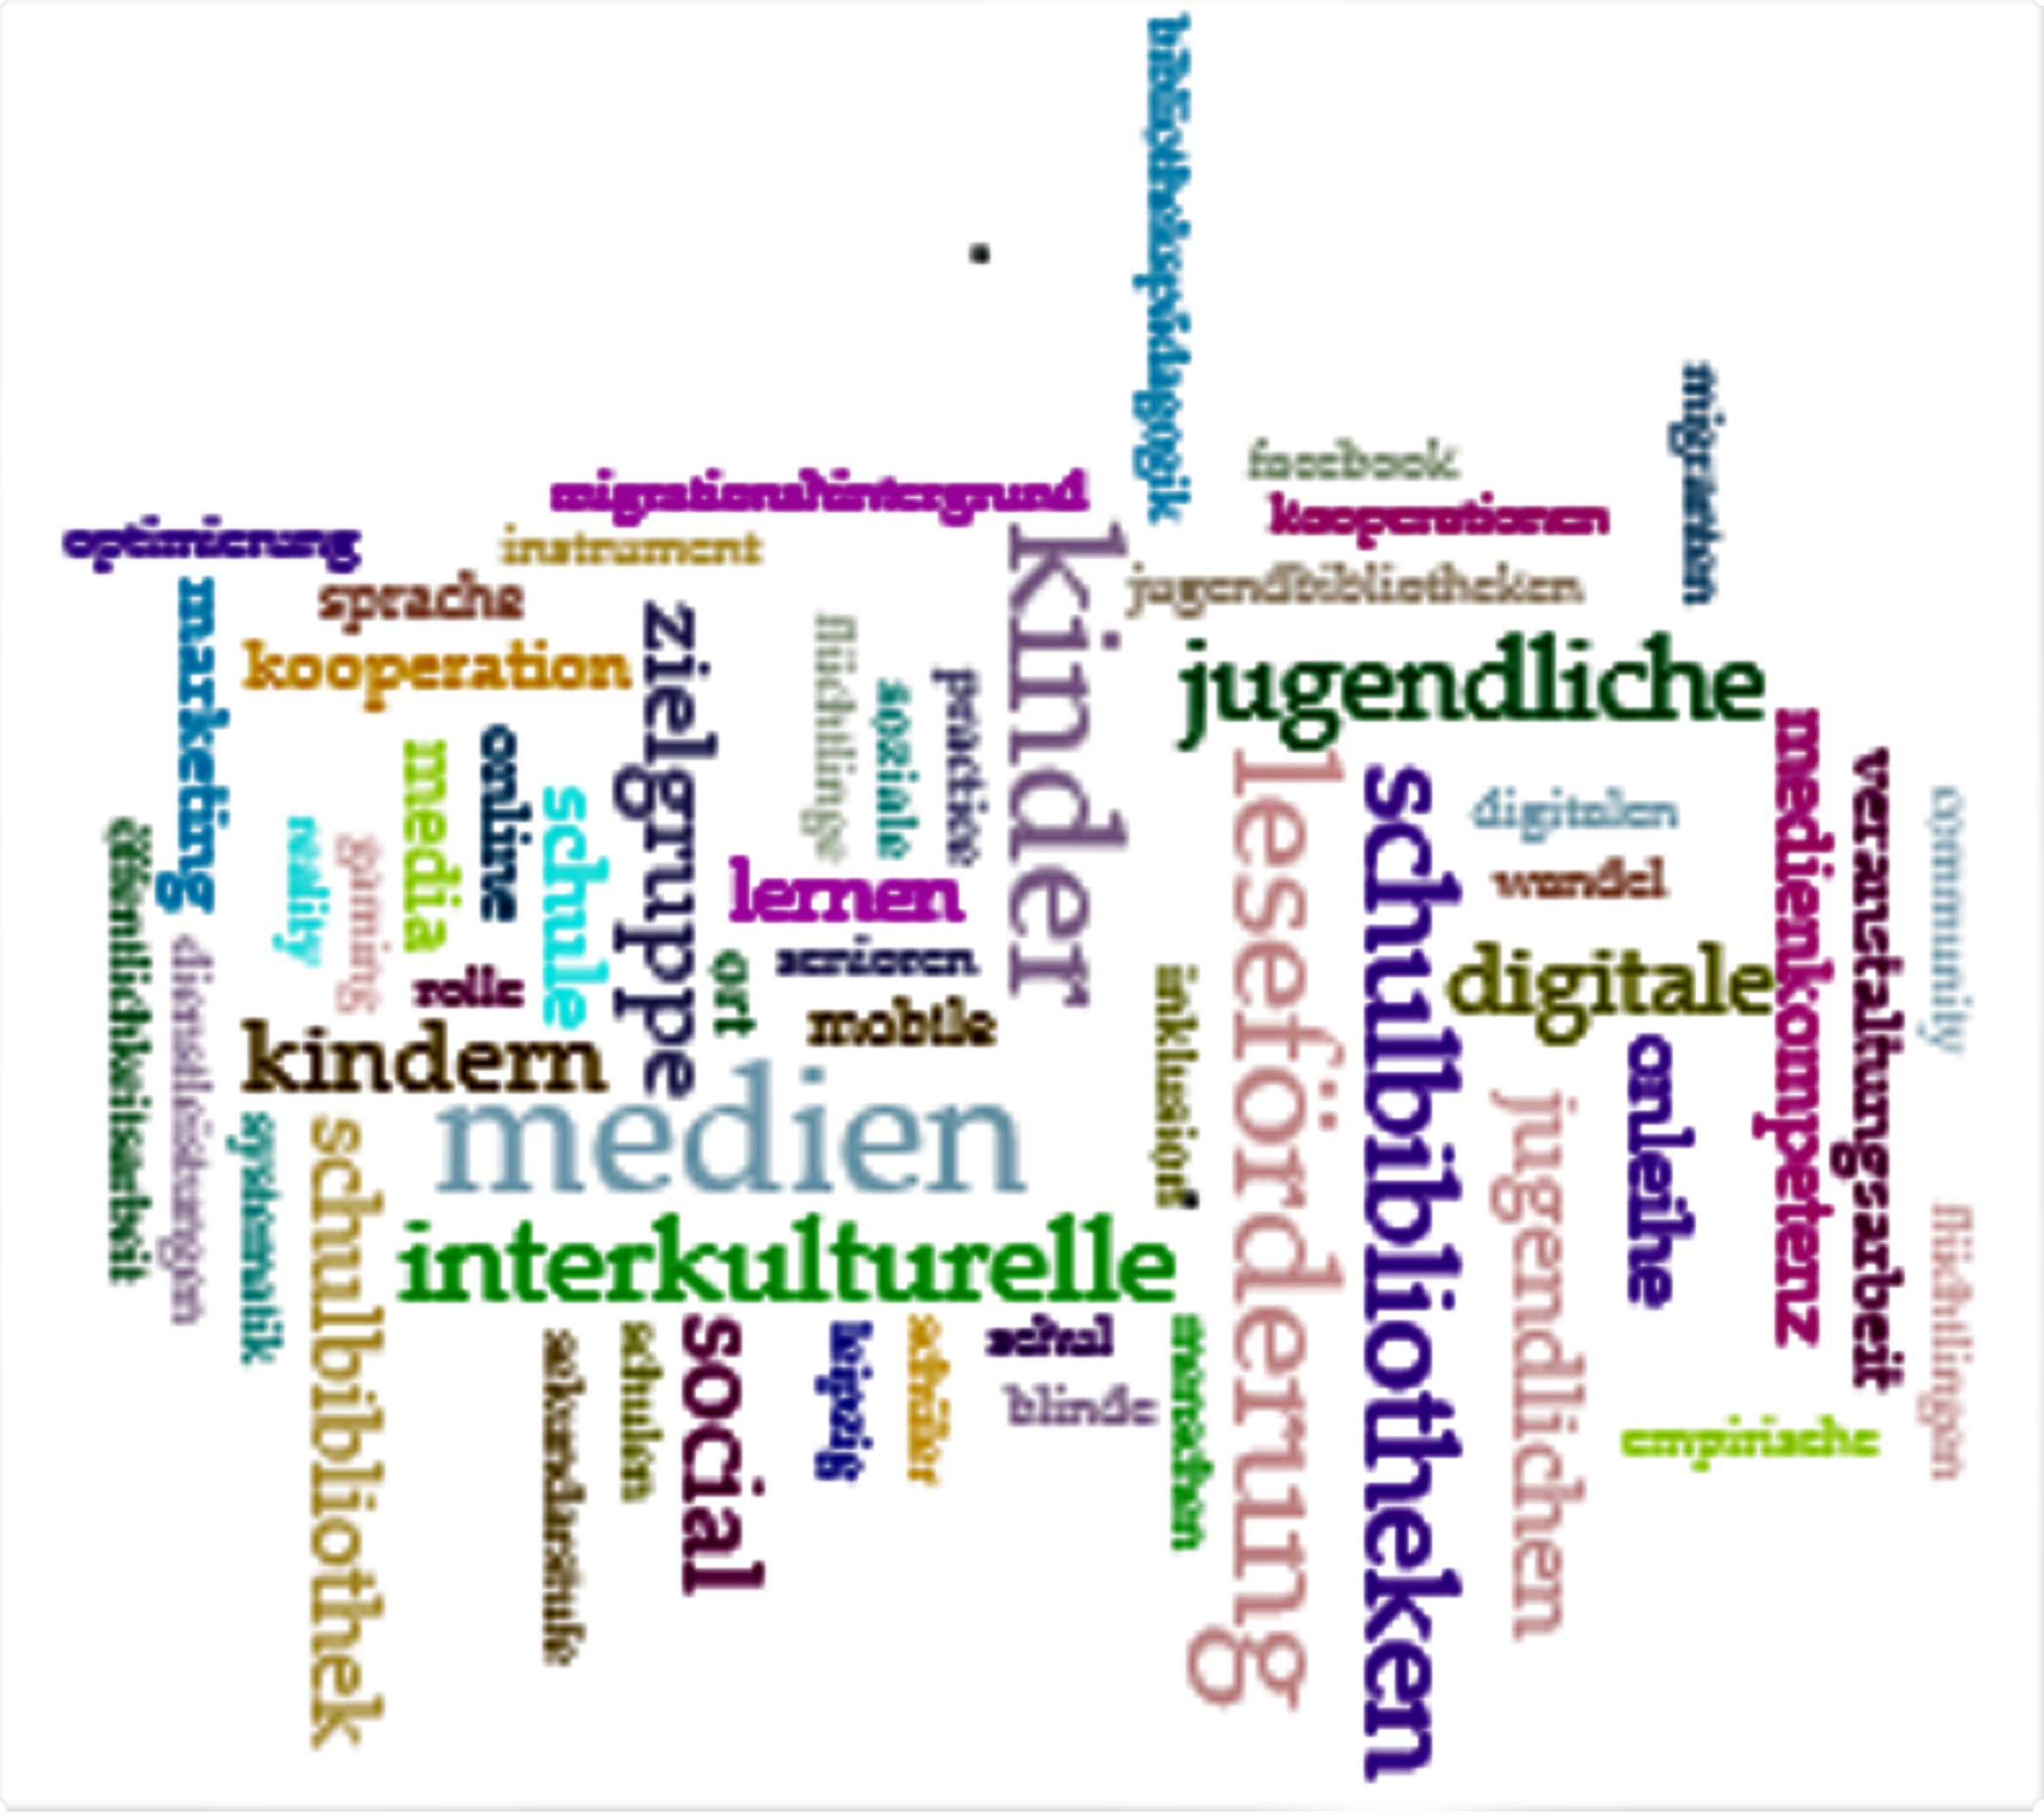
\includegraphics{img/image1.png}
\caption{Wortwolke aus Titeln von ca. 550 Abschlussarbeiten mit ÖB-Bezug
2010--2019}
\end{figure}

Die Wortwolke weist darauf hin, dass sich die Abschlussarbeiten im
Bereich der Öffentlichen Bibliotheken zu einem erheblichen Teil mit
Kindern und Jugendlichen und Bibliotheksangeboten für sie beschäftigen
und sich im Bereich der Leseförderung, der Medienkompetenz und des
Lernens bewegen. Weitere Themen, die in der Wortwolke sichtbar werden,
sind besondere Zielgruppen wie Geflüchtete und ausgerechnet
Schulbibliotheken, die im Bibliotheksfeld Deutschlands eine
ausgesprochene Randlage einnehmen.

Als neuer, zentraler Faktor seit 2000 (der ersten Pisa-Studie) zeigt
sich also in der Forschung zu Öffentlichen Bibliotheken (wie auch im
Fachdiskurs, vergleiche Wimmer 2019a: 278--279) eine starke Fokussierung
auf das Kind als Bibliotheksnutzer. Damit einher geht auch eine neue
wissenschaftliche Angrenzung an die Erziehungswissenschaft, die erstmals
im Sammelband 2005 auftauchte (Lernarragements) und auch bei Lankes
anklingt. Es scheint, dass sich die Öffentlichen Bibliotheken als
Einrichtungen für Kinder positionieren.

Überhaupt nicht zu sehen ist hier der betriebswirtschaftliche Aspekt
(außer vielleicht in den Termen Öffentlichkeitsarbeit und Kooperation).
Nach wie vor präsent -- allerdings nur noch in abstrakter Form -- ist
das \enquote{Bibliotheksgut}: Medien, vor allem in digitalen Medien, zum
Beispiel in der Onleihe.

\hypertarget{fazit}{%
\section{Fazit}\label{fazit}}

Die Untersuchung zeigte, dass sich Forschung zu Öffentlichen
Bibliotheken in Deutschland ursprünglich den drei Bereichen

\begin{itemize}
\item
  NutzerInnen/ Soziologie,
\item
  Inhalte/ Medien/ Programme/ Medien- oder Kommunikationswissenschaft
  und
\item
  Bibliotheksbetrieb / Betriebswirtschaftslehre
\end{itemize}

zuordnen ließ. Die meisten der auf Öffentliche Bibliotheken bezogenen
Forschungsdesiderate und -programme lassen sich mehr oder weniger
offensichtlich einem dieser drei Bereiche zuordnen.

Besonders wichtig ist aber, dass als viertes Zielsystem an allen
untersuchten Stationen ein Kollektiv als Zielsystem der
Bibliotheksarbeit avisiert wurde: das Volk, die Gesellschaft, und
neuerdings die Community. Insofern ist ein soziologischer Ansatz für die
Wissenschaft von der Öffentlichen Bibliothek prägend und durchgängig
sichtbar (und sie unterscheidet sich dadurch deutlich von den
wissenschaftlichen Bibliotheken, in denen der Community-Begriff erst in
den letzten Jahren aufgetaucht ist). In den Theorien der 2010er Jahre
(Lankes, Aundson und Jochumson) steht ausschließlich der soziologische
Ansatz im Mittelpunkt.

Das \enquote{Bibliotheksgut} -- also Medien und Inhalte, auch unter
kommunikations- und medienwissenschaftlichem Ansatz betrachtet, ist im
Lauf der Zeit immer abstrakter und weniger präsent geworden: Vom
zentralen Instrument der BibliothekarInnen, zielgerecht eingesetzt zur
Bildung der LeserInnen bei Hofmann, zu einem Medium der
gesellschaftlichen \enquote{Kommunikation} bei Henning, bis zu Lankes,
wo die physischen Medien weitgehend durch Interaktion zwischen Menschen
ersetzt werden.

Der betriebs- und volkswirtschaftliche Bereich war in den 1920er und
1970er Jahren als konstitutiver Teil der Bibliothekswissenschaft sehr
präsent und auch im 2005er Kompendium noch vertreten. 2018 taucht er
jedoch überhaupt nicht mehr auf. Das ist erstaunlich, wenn man bedenkt,
dass betriebswirtschaftliche Instrumente seitens der Kommunen seit
Anfang der 1990er Jahre flächendeckend eingesetzt wurden. Eine Erklärung
könnte darin liegen, dass die Instrumente nun realisiert sind (und nicht
mehr besprochen werden müssen), dass dieses Thema in der ökonomisch
entspannten Situation der 2010er Jahre nicht drängend ist -- oder dass
im 2018er Sonderheft keine Praktiker sprechen. Wann immer diese zu Wort
kommen, wird die \enquote{Zentrale Forschungsfrage} -- nach dem Beweis
der Wirkung der Bibliothek -- explizit oder implizit geäußert.

Auffällig ist die starke Präsenz des Kindes im Fachdiskurs und in den
Abschlussarbeiten seit 2010 -- nicht jedoch in den untersuchten
Forschungsprogrammen (außer als \enquote{Lernende}).

Aufschlussreich ist auch, welche Themen in den untersuchten Programmen
\emph{fehlen}. Das sind zum Beispiel:

\begin{itemize}
\item
  technische Entwicklungen
\item
  Erschließungsthemen (jedoch unter entwicklungspsychologischen Aspekten
  bei Hofmann)
\item
  Erwerbungsfragen
\item
  Sammeln, Erschließen, Bewahren
\item
  Auch der Begriff Information taucht verhältnismäßig sparsam in allen
  untersuchten Texten auf.
\end{itemize}

Die zentralen Punkte der bibliothekarischen Tätigkeit in
wissenschaftlichen Bibliotheken und der klassischen
Bibliothekswissenschaft im Sinne einer Informationswissenschaft spielen
in den Forschungsprogrammen für die Öffentlichen Bibliotheken also
praktisch keine Rolle.

In Teil 1 dieses Beitrags wurde auf das Verhältnis zwischen Akademie und
Profession, zwischen Forschung und Management eingegangen. Ergebnisse
dieser Überlegungen waren unter anderem, dass es sich um zwei
unterschiedliche Handlungsfelder mit jeweils anderen Aufgaben und Rollen
handelt, und dass Ergebnisoffenheit Primat der Forschung ist,
Erfolgsorientierung Primat des Managements. Parteinahme von
ForscherInnen für Öffentliche Bibliotheken äußert sich dadurch, dass
Öffentliche Bibliotheken und ihre NutzerInnen als Forschungsgegenstand
gewählt werden.

Wie verhalten sich diese Überlegungen zu den Ergebnissen aus Teil 2?
Zunächst hat sich gezeigt, dass das Konzept der getrennten
Handlungsfelder nicht durchgängig beobachtet werden kann. Am klarsten
präsent war es in der Situation der Akademisierung (FHB-Colloquium 1974)
-- hier sprachen Akademiker \emph{und Praktiker} für Grundlagenforschung
-- und im Sonderheft 2018 von \enquote{Bibliothek Forschung und Praxis},
in dem es einen (fast) rein akademischen Diskurs gibt. Dagegen zeigt
sich aus Sicht der Profession immer wieder ein ganz anderes Modell
(besonders explizit im Beitrag von Klaus-Peter Böttger 2005): eine
Beratungs- und Unterstützungsrolle der Hochschulen für die
Bibliothekspraxis, die auf einer besonders \enquote{engen und
vertrauensvollen} Beziehung zwischen beiden beruht. Neben dem Gegensatz
zwischen Ergebnisoffenheit und Erfolgsorientierung könnten diese beiden
verschiedenen Vorstellungen ein Grund für viele Missverständnisse und
Rollenkonflikte zwischen Akademie und Profession sein -- und ein Ansatz,
um sie zu thematisieren und zu bearbeiten.

Des weiteren fällt auf, dass die aktuellen Abschlussarbeiten an den
Hochschulen weit mehr Aspekte behandeln, die der Agenda der
\emph{Bibliothekspraxis} zuzuordnen sind (Kinder, Jugendliche, Neue
Medien), als die, die im Themenheft \enquote{Bibliothek Forschung und
Praxis} genannt sind. Selbstverständlich wählen sich Mittzwanziger
BerufseinsteigerInnen andere Forschungsthemen als Mittfünfziger
Akademiker. Aber trotzdem zeigt sich hier, dass der Bezug zwischen
beiden Handlungsfeldern nach wie vor stark ist und in viele aktuelle
Forschungsprojekte hinein wirkt.

\hypertarget{ausblick}{%
\section{Ausblick}\label{ausblick}}

Auf der Basis der Untersuchung können wir die Zuordnung von Forschung zu
den drei \enquote{klassischen} Bereichen: Soziologie -- Medien/ Inhalt
-- Betriebswirtschaft nun jeweils genauer untersuchen. Besonders
interessant wäre das in Bezug auf den soziologischen Ansatz. Ihm stand
die Wissenschaft von der Öffentlichen Bibliothek von Anfang an am
nächsten. Die konkrete Ausrichtung dieses soziologischen Ansatzes hat
sich aber sehr geändert. Es wäre sinnvoll zu untersuchen, welche Art
Soziologie und welche Aspekte und Fragestellungen im Lauf der Zeit sich
hinter dem Begriff \enquote{Bibliothekssoziologie} verbargen.

Die Auswertung der Abschlussarbeiten, die hier nur skizziert werden
konnte, wird in einem folgenden Beitrag fortgesetzt und vervollständigt.

Auf die Ausrichtung der Forschung zu Öffentlichen Bibliotheken in
anderen Ländern (insbesondere Skandinavien, GB und USA) konnte hier
nicht mehr eingegangen werden; dies wäre ein relevanter nächster
Schritt.

\hypertarget{literatur}{%
\section{Literatur}\label{literatur}}

Beyersdorff, Günter 1974. Von der Allgemeinen Beitriebswirtschaftslehre
zu einer Bibliotheksbetriebslehre. Erste Erfahrungen bei einer
betriebswirtschaftlichen Untersuchung Öffentlicher Bibliotheken. In
Bibliothekswissenschaft und Öffentliche Bibliothek. Referate und
Ergebniszusammenfassungen eines Fortbildungsseminars der FHB Stuttgart.
Bibliotheksdienst Beiheft. Berlin: Deutscher Bibliotheksverband,
Arbeitsstelle für das Bibliothekswesen, 23--38.

Boese, Engelbrecht 1981. Walter Hofmanns \enquote{Institut für Leser-
und Schrifttumskunde} 1926-1937. BIBLIOTHEK Forschung und Praxis 5, 1,
3--23.

Böttger, Klaus-Peter 2005. Öffentliche Bibliotheken und die
Bibliothekswissenschaft - Eine persönliche Einschätzung. In
\emph{Bibliothekswissenschaft - quo vadis? Eine Disziplin zwischen
Traditionen und Visionen: Programme - Modelle - Forschungsaufgaben}.
Berlin, Boston: De Gruyter Saur, 295--300.

Emunds, Heinz 1974. Bibliotheksleistungen. Empirische Beiträge im
Vorfeld der Bibliothekswissenschaft. In Bibliothekswissenschaft und
Öffentliche Bibliothek. Referate und Ergebniszusammenfassungen eines
Fortbildungsseminars der FHB Stuttgart. Bibliotheksdienst Beiheft.
Berlin: Deutscher Bibliotheksverband, Arbeitsstelle für das
Bibliothekswesen, 39--58.

Dankert, Birgit 2005. Immer wieder sonntags - Zur Didaktik
schulbibliothekarischer Arbeit. In Bibliothekswissenschaft - quo vadis?
Eine Disziplin zwischen Traditionen und Visionen: Programme - Modelle -
Forschungsaufgaben. Berlin, Boston: De Gruyter Saur, 301--312.

Harari, Yuval Noaḥ 2018. Eine kurze Geschichte der Menschheit. 30.
Auflage. München: Pantheon.

Hauke, Petra (Hg.) 2005. Bibliothekswissenschaft - quo vadis?: eine
Disziplin zwischen Traditionen und Visionen: Programme - Modelle -
Forschungsaufgaben. Berlin, Boston: DeGruyter Saur.
\url{http://dx.doi.org/10.1515/9783110929225}.

Heidtmann, Frank 1974. Die bibliothekarische Berufswahl. Pullach: Verlag
Dokumentation.

Henning, Wolfram 1974. Öffentliche Bibliothek und soziale Kommunikation.
In Bibliothekswissenschaft und Öffentliche Bibliothek. Referate und
Ergebniszusammenfassungen eines Fortbildungsseminars der FHB Stuttgart.
Bibliotheksdienst Beiheft. Berlin: Deutscher Bibliotheksverband,
Arbeitsstelle für das Bibliothekswesen, 95--121.

Hobohm, Hans-Christoph 2018. Warum brauchen wir eine (neue)
Bibliothekswissenschaft?: Editorial. Bibliothek Forschung und Praxis 42,
2, 333--337.

Hofmann, Walter 1911. Bildung und Ausbildung des Volksbibliothekars. In:
Archiv für Volksbildung, Heft 2. Nachdruck in: Buch und Volk. Gesammelte
Aufsätze und Reden zur Buchpolitik und Volksbüchereifrage. Köln: Verlag
Der Löwe, 1951, S. 121--129.

Hohlfeld, Klaus 1974. Die Öffentliche Bibliothek in einer menschlichen
Stadt. Aufforderung zu einer Diskussion. Buch und Bibliothek 26,
270--276.

Institut für Arbeitsmarkt-und Berufsforschung (2020). \enquote{Berufe im
Spiegel der Statistik.}
\url{http://bisds.iab.de/Default.aspx?beruf=BG733\&region=1\&qualifikation=0}
(Zugriff am 11.04.2020).

Jochumsen, Henrik 2018. How to Qualify the Debate on the Public Library
by the Use of Re\-search-Developed Tools. Bibliothek Forschung und Praxis
42, 2, 344--350.

Klotzbücher, Alois 1974. Benutzerforschung als Aufgabe einer neuen
Bibliothekswissenschaft. In Bibliothekswissenschaft und öffentliche
Bibliothek: Referate und Ergebniszusammenfassungen eines
Fortbildungsseminars der FHB Stuttgart. Bibliotheksdienst Beiheft.
Berlin: Deutscher Bibliotheksverband, Arbeitsstelle für das
Bibliothekswesen, 59--76.

König-Kurowski, Gerhard 1974. Benutzerforschung und
Bibliothekssoziologie. In Bibliothekswissenschaft und öffentliche
Bibliothek: Referate und Ergebniszusammenfassungen eines
Fortbildungsseminars der FHB Stuttgart. Bibliotheksdienst Beiheft.
Berlin: Deutscher Bibliotheksverband, Arbeitsstelle für das
Bibliothekswesen, 77--94.

Koop, Ulrike 2017. Wertzumessung für Öffentliche Bibliotheken.
\url{https://doi.org/10.18452/18125}.

L., P. 1928. Institut für Leser- und Schrifttumskunde. Hefte für
Büchereiwesen 12, 3, 171--174.

Lankes, R. David 2011. The Atlas of New Librarianship. Cambridge, Mass:
MIT Press.

Lux, Claudia 2005. Braucht die Praxis die Bibliothekswissenschaft? In
Bibliothekswissenschaft - quo vadis? Eine Disziplin zwischen Traditionen
und Visionen: Programme - Modelle - Forschungsaufgaben. Berlin, Boston:
De Gruyter Saur, 287--294.

Moeske, Ulrich 2005. Kosten-Leistungsrechnung in Bibliotheken - Ihre
Auswirkung auf Organisation und Finanzen. In Bibliothekswissenschaft -
quo vadis? Eine Disziplin zwischen Traditionen und Visionen: Programme -
Modelle - Forschungsaufgaben. Berlin, Boston: De Gruyter Saur, 345--362.

o.\,A. 1974a. Bibliothekswissenschaft und öffentliche Bibliothek:
Referate und Ergebniszusammenfassungen eines Fortbildungsseminars der
FHB Stuttgart. Berlin: Deutscher Bibliotheksverband, Arbeitsstelle für
das Bibliothekswesen.

o.\,A. 1974b. Kurze Zusammenfassung der Diskussionsergebnisse beim
Stuttgarter Seminar \enquote{Bibliothekswissenschaft und Öffentliche
Bibliothek.} In Bibliothekswissenschaft und öffentliche Bibliothek:
Referate und Ergebniszusammenfassungen eines Fortbildungsseminars der
FHB \linebreak Stuttgart. Bibliotheksdienst Beiheft. Berlin: Deutscher
Bibliotheksverband, Arbeitsstelle für das Bibliothekswesen, 123--126.

o.\,A. Paneldiskussion: Öffentliche Bibliotheken in Forschung und Lehre
--- Institut für Biblio\-theks- und Informations­wissen­schaft.
\url{https://www.ibi.hu-berlin.de/de/online-archiv/veranstaltungen/paneldiskussionoeb}
{[}Stand 2020-03-26{]}.

Ochudlo-Höbing, Kerstin 2005. E-Learning für Jugendliche und junge
Erwachsene - Eine Herausforderung für Öffentliche Bibliotheken. In
Bibliothekswissenschaft - quo vadis? Eine Disziplin zwischen Traditionen
und Visionen: Programme - Modelle - Forschungsaufgaben. Berlin, Boston:
De Gruyter Saur, 325--344.

Reuveni, Gideon 2013. Lesen im Nachkriegsdeutschland.
Geschichtsliteratur in der Weimarer Republik - eine Fallstudie. In
Archiv für Geschichte des Buchwesens. Walter de Gruyter, 203--225.

Rohde, Renate 2004. Zur Geschichte der bibliothekswissenschaftlichen
Ausbildung in Berlin. \url{http://www.ib.hu-berlin.de/inf/geschbw.htm}
{[}Stand 2020-03-30{]}.

Saalmann, Gernot 2014. Emile Durkheim. In Bourdieu-Handbuch. Leben -
Werk - Wirkung. Stuttgart: Metzler, 32--36.

Schütz, Alfred 1971. Gesammelte Aufsätze. 1, Das Problem der sozialen
Wirklichkeit.

Schwarz, Helga 2018. Das Deutsche Bibliotheksinstitut im Spannungsfeld
zwischen Auftrag und politischen Interessen. Berlin: Simon Verlag für
Bibliothekswissen.

Süle, Tibor 1972. Bücherei und Ideologie: Politische Aspekte im
Richtungsstreit deutscher Volksbibliothekare 1910-1930. Köln: Greven.

Ulrich, Paul S. 2005. The Library as a Real - Virtual - Public Place for
Networking Ideas, Information and People. In Bibliothekswissenschaft -
quo vadis? Eine Disziplin zwischen Traditionen und Visionen: Programme -
Modelle - Forschungsaufgaben. Berlin, Boston: De Gruyter Saur, 191--206.

Veit, Annegret 2002. Professionelles Handeln als Mittel zur Bewältigung
des Theorie-Praxis-Problems in der Krankenpflege. Universität Leipzig,
Leipzig.

Vodosek, Peter 1981. \enquote{Zur Entwicklung des bibliothekarischen
Berufs als Frauenberuf.} In: BIBLIOTHEK Forschung und Praxis. 5 (3), S.
231--244.

Vodosek, Peter 2006. Innovation und Ideologie. Walter Hofmann und sein
Büchereiwerk in Dresden-Plauen und Leipzig. Lifelong education and
libraries 6, 9--29.

Wimmer, Ulla 2019a. Die Geschichte vom großen Ö. Die Position der
Öffentlichen Bibliotheken im Bibliotheksfeld und im bibliothekarischen
Fachdiskurs der Bundesrepublik Deutschland seit 1964. Berlin:
Humboldt-Universität. \url{https://doi.org/10.18452/19791}.

Wimmer, Ulla 2019b. Rasender Stillstand: Die Gender-\enquote{Speech-Gap}
in Bibliotheken.
\url{https://nbn-resolving.org/urn:nbn:de:0290-opus4-165902} {[}Stand
2020-03-24{]}.

Wimmer, Ulla 2019c. Wo sind die Öffentlichen Bibliotheken in Forschung
und Lehre?. In: Hauke, Petra (Hg). Öffentliche Bibliothek 2030:
Herausforderungen-Konzepte-Visionen. Bad Honnef: Bock + Herchen Verlag.
\url{https://doi.org/10.18452/20169}.

%autor
\begin{center}\rule{0.5\linewidth}{0.5pt}\end{center}

\textbf{Ulla Wimmer} ist wissenschaftliche Mitarbeiterin am Institut für
Bibliotheks- und Informationswissenschaft der Humboldt-Universität zu
Berlin. Nach Abschluss als Diplom-Bibliothekarin (ÖB) an der FU Berlin
war sie im Deutschen Bibliotheksinstitut, in der Stadtbibliothek
Berlin-Neukölln und beim Deutschen Bibliotheksverband tätig, bevor sie
2012 zur HU wechselte. 2003 MA in Kulturwissenschaft und
Betriebswirtschaft. 2018 Promotion am IBI zum Thema ``Die Geschichte vom
großen Ö: die Position der Öffentlichen Bibliotheken im Bibliotheksfeld
und im bibliothekarischen Fachdiskurs''. Lehrgebiete und
Forschungsinteressen: Management-, kulturwissenschaftliche, historische
und soziologische Aspekte von Bibliothek und Information, Feld- und
Professionssoziologie, Genderfragen sowie quantitative Methoden, Messen
und Statistik.

\end{document}
